\chapter{Compressori assiali}

\section{Introduzione}
I compressori assiali sono macchine relativamente recenti; si tratta infatti di macchine nate nel dopoguerra come componente per i gruppi turbina a gas in campo aeronautico. I primi motori aeronautici costituiti da gruppo turbogas sono stati inizialmente costruiti come compressori radiali; oggi in qualsiasi gruppo turbogas, salvo gruppo di dimensioni molto ridotte, si utilizzano compressori assiali.
\begin{figure}[h!]
\centering
  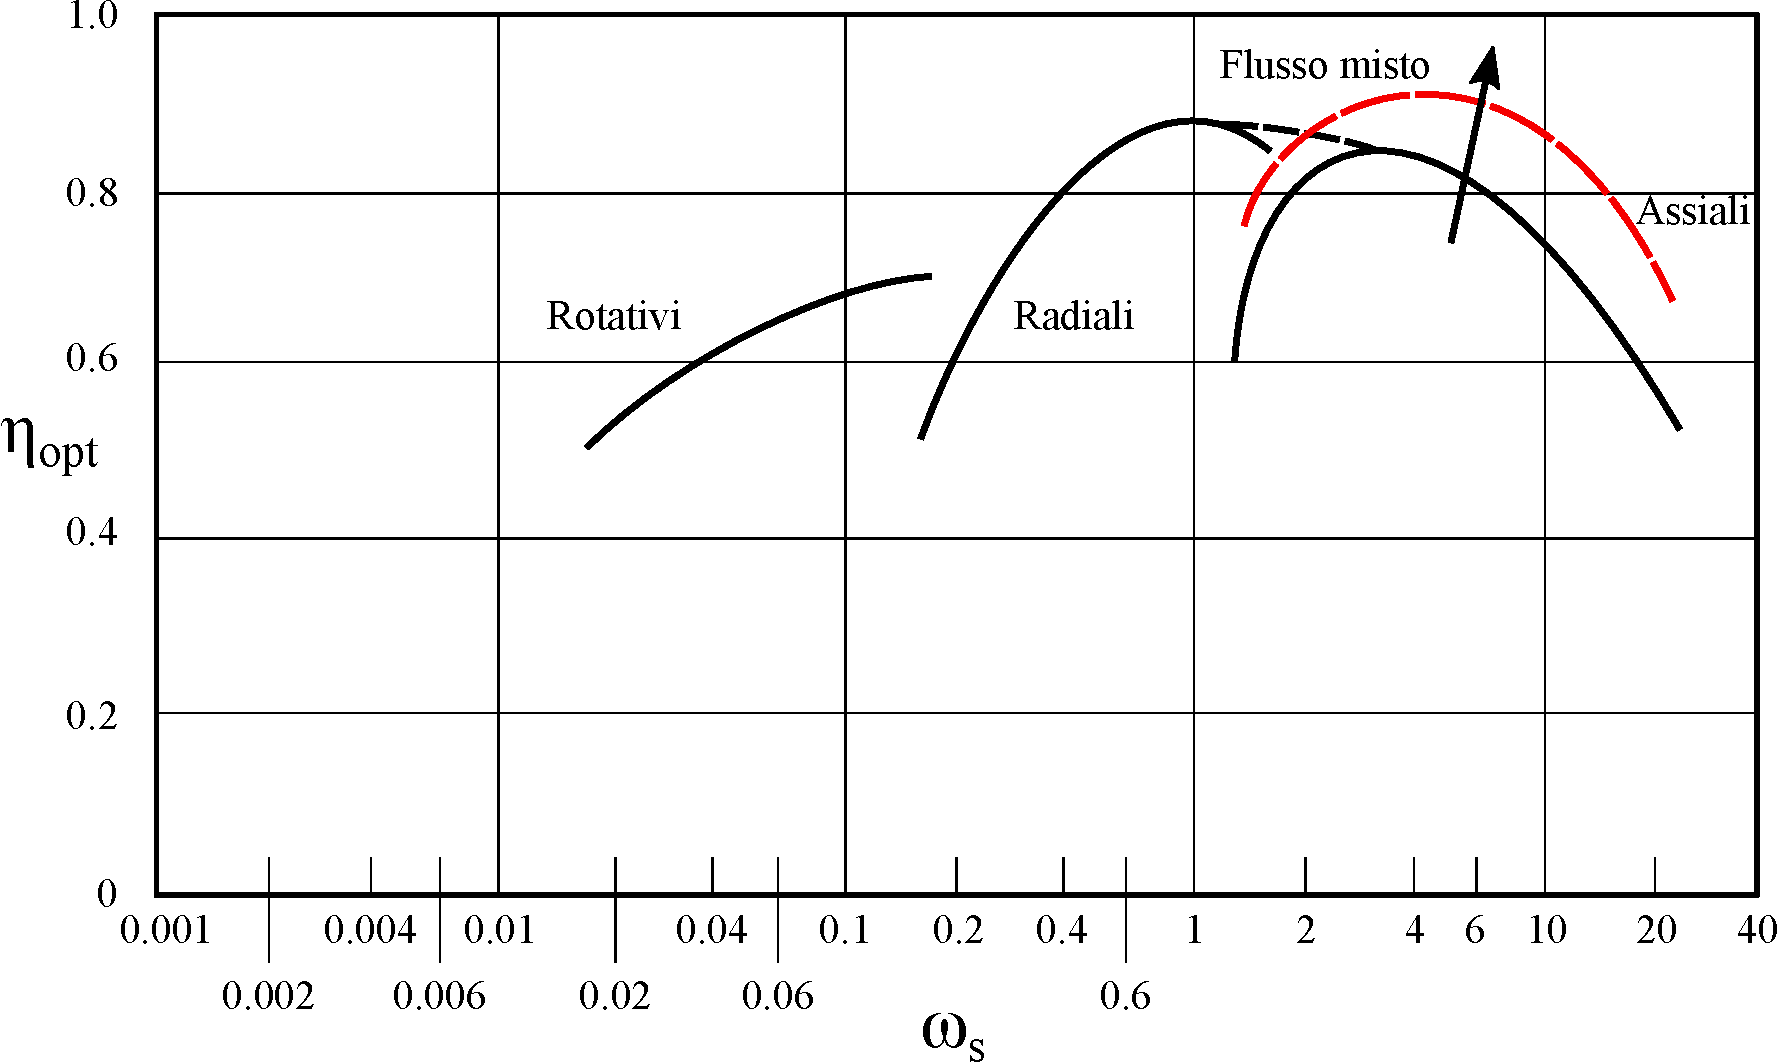
\includegraphics[width=.8\textwidth]{fig/PrestComp.pdf}
\caption{A destra le curve di rendimento per le macchine assiali. Si nota l'evidente aumento delle prestazioni (in rosso le curve per le macchine attuali) rispetto alle prime macchine.}
\label{fig:PrestComp}
\end{figure}

C'è una forte correlazione tra compressione ottenibile e rendimento. Nel diagramma in figura \ref{fig:PrestComp} è presente il rendimento del compressore in funzione della velocità specifica $\omega_s$ (che rappresenta la caratteristica di macchina) definita a partire dal coefficiente di carico $\psi$ e dal coefficiente di portata $\varphi$ ($S$ è la sezione anulare di passaggio di diametri $D_e$ e $D_i$):
\begin{align*}
\psi = \cfrac{\Delta h_{0is}}{\cfrac{u^2}{2}} \hspace{2cm} \varphi = \frac{Q}{u \cdot S}
\end{align*}
\begin{align*}
\omega_s = \cfrac{\sqrt{\varphi}}{\psi^{3/4}} \cdot \sqrt{\bigg( \cfrac{D_e}{D_i} \bigg)^2 -1}
\end{align*}
Si nota che all'aumentare della velocità specifica si va verso macchine assiali.

Fino ad un certo punto della storia le macchine assiali non hanno goduto di rendimenti competitivi; in rosso (figura \ref{fig:PrestComp}) è presentata la curva dello stato attuale dei rendimenti per macchine assiali che si vede essere maggiore rispetto quello delle prime macchine di questa tipologia. 
\begin{figure}
\centering
  \includegraphics[width=.4\textwidth]{fig/hsComp.pdf}
\caption{1: ingresso statore 2: uscita statore - entrata rotore 3: uscita statore.}
\label{fig:hsComp}
\end{figure}
\\Nel diagramma termodinamico in figura \ref{fig:hsComp} sono riportati gli stati di riferimento di uno stadio di compressore assiale. Nella parte rotorica avviene il lavoro con un relativo aumento della velocità mentre nello statore c'è il recupero in termini di pressione. Nello studio delle macchine assiali vengono fatte generalmente le seguenti assunzioni:
\begin{itemize}
\item flusso adiabatico, visto il tempo di contatto fluido-paletta molto limitato;
\item stadio ``normale" o ``ripetuto", tutti gli stadi hanno gli stessi profili:
\begin{align*}
c_1 = c_2 \;\;\;\; \Rightarrow \;\;\;\; h_3-h_1 = h_{03} - h_{01}
\end{align*}
\item velocità assiale costante (coincide con la velocità meridiana):
\begin{align*}
c_{m1} = c_{m2}
\end{align*}
\item densità costante nello stadio:
\begin{align*}
\rho = cost
\end{align*}
\end{itemize}
\section{Lavoro e triangoli di velocità}
Nel rotore si conserva la rotalpia:
\begin{equation}
h_1 + \frac{1}{2} w_1^2 = h_2 + \frac{1}{2} w_2^2
\end{equation}
Nello statore si conserva l'entalpia:
\begin{equation}
h_2 + \frac{1}{2} c_2^2 = h_3 + \frac{1}{2} c_3^2
\end{equation}
Il lavoro viene scambiato dalla parte rotorica e si definisce un parametro adimensionale per quest'ultimo ($u$ rimane costante visto che si sta trattando una macchina assiale, c'è una differenza rispetto la precedente definizione di lavoro adimensionale data da un fattore 1/4):
\begin{equation}
\lambda = \frac{u \cdot c_{u2} - u \cdot c_{u1}}{u^2} = \frac{c_{u2} - c_{u1}}{u}
\end{equation}
\begin{figure}
\centering
  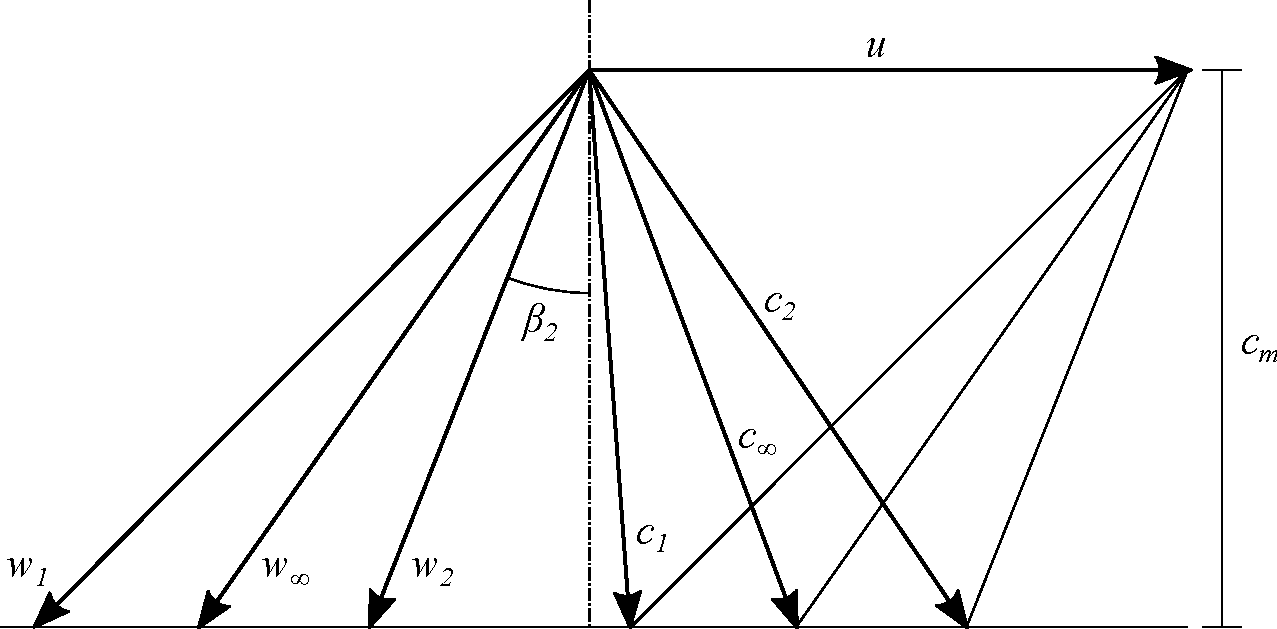
\includegraphics[width=.8\textwidth]{fig/triangComp.pdf}
\caption{}
\label{fig:triangComp}
\end{figure}
\\L'obiettivo è quello di determinare la relazione tra $\lambda$ e cifra di portata $\Phi$ definita come:
\begin{align*}
\Phi = \frac{c_m}{u}
\end{align*}
Si disegnano i triangoli di velocità relativi allo stadio elementare come mostrato in figura \ref{fig:triangComp}; per definizione la componente meridiana e periferica sono costanti. Si possono scrivere le seguenti tre relazioni:
\begin{align*}
c_{u2} = u - w_{u2}
\end{align*}
\begin{align*}
w_{u2} = c_m \tan \beta_2
\end{align*}
\begin{align*}
c_{u1} = c_m \tan \alpha_1
\end{align*}
e quindi scrivere:
\begin{align*}
\lambda = 1- \frac{w_{u2}}{u} - \frac{c_{u1}}{u} = 1 - \frac{c_m}{u} \left(\tan \beta_2 + \tan \alpha_1 \right)
\end{align*}
\'E possibile scrivere la cifra adimensionale relativa al lavoro scambiato dalla parte rotorica in funzione della cifra di portata come:
\begin{equation}
\lambda = 1 - \Phi \left( \tan \beta_2 + \tan \alpha_1 \right) = 1 - k \cdot \Phi
\end{equation}
con $k$ costante che dipende dalla geometria della macchina. Si tratta di una rappresentazione molto simile a quella del caso delle pompe centrifughe nelle quali, a seconda del valore di $k$, si ha la curva caratteristica della pompa; questo viene chiarito meglio dal diagramma in figura \ref{fig:CondProg}.
\begin{figure}
\centering
  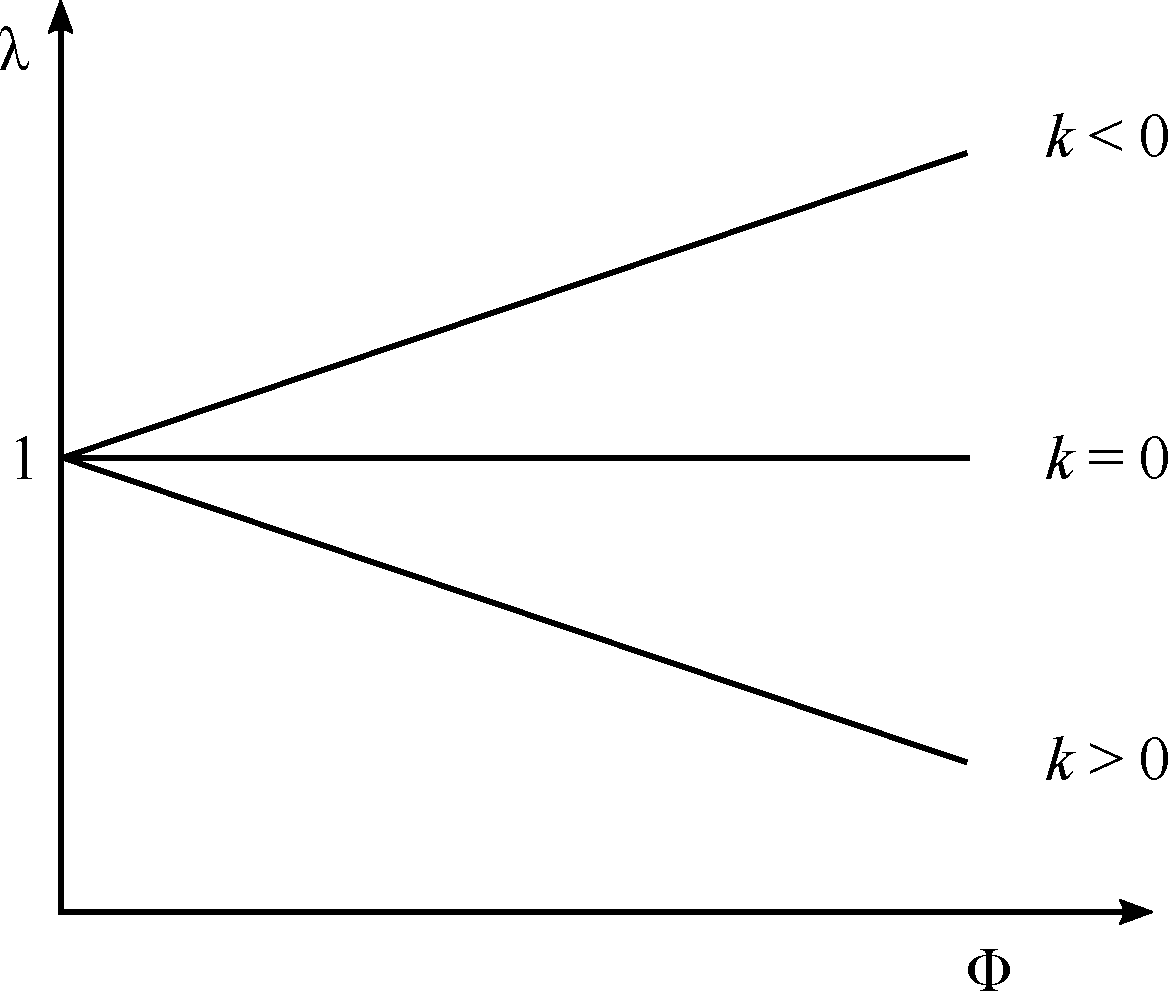
\includegraphics[width=.4\textwidth]{fig/CondProg.pdf}
\caption{}
\label{fig:CondProg}
\end{figure}
\\Si definisce una condizione particolare di progetto ``lambda di design" $\lambda_d$:
\begin{align*}
\lambda_d = 1 - k \cdot \Phi_d \;\;\;\; \rightarrow \;\;\;\; k = \frac{1}{\Phi_d}-\frac{\lambda_d}{\Phi_d}
\end{align*}
Sostituendo l'espressione di $k$ qui ricavata nella definizione generale di $\lambda$, si ottiene:
\begin{equation} \label{eq:lambdad}
\frac{\lambda}{\lambda_d} = \frac{1}{\lambda_d} - \frac{\Phi}{\Phi_d} \Bigg( \frac{1-\lambda_d}{\lambda_d} \Bigg) \;\;\;\; \text{con}\; 0.3 < \lambda_d < 0.4
\end{equation}
Si tratta di una famiglia di rette; in figura \ref{fig:LambdaPhiChart} è rappresentato il diagramma caratteristico espresso in termini di rapporti rispetto alle condizioni di progetto. Nel caso ideale di $\lambda_d = 1$ il lavoro scambiato sarebbe indipendente dalla portata, situazione abbastanza attraente ma irrealizzabile. 
\begin{figure}
\centering
\begin{minipage}{.5\textwidth}
  \centering
  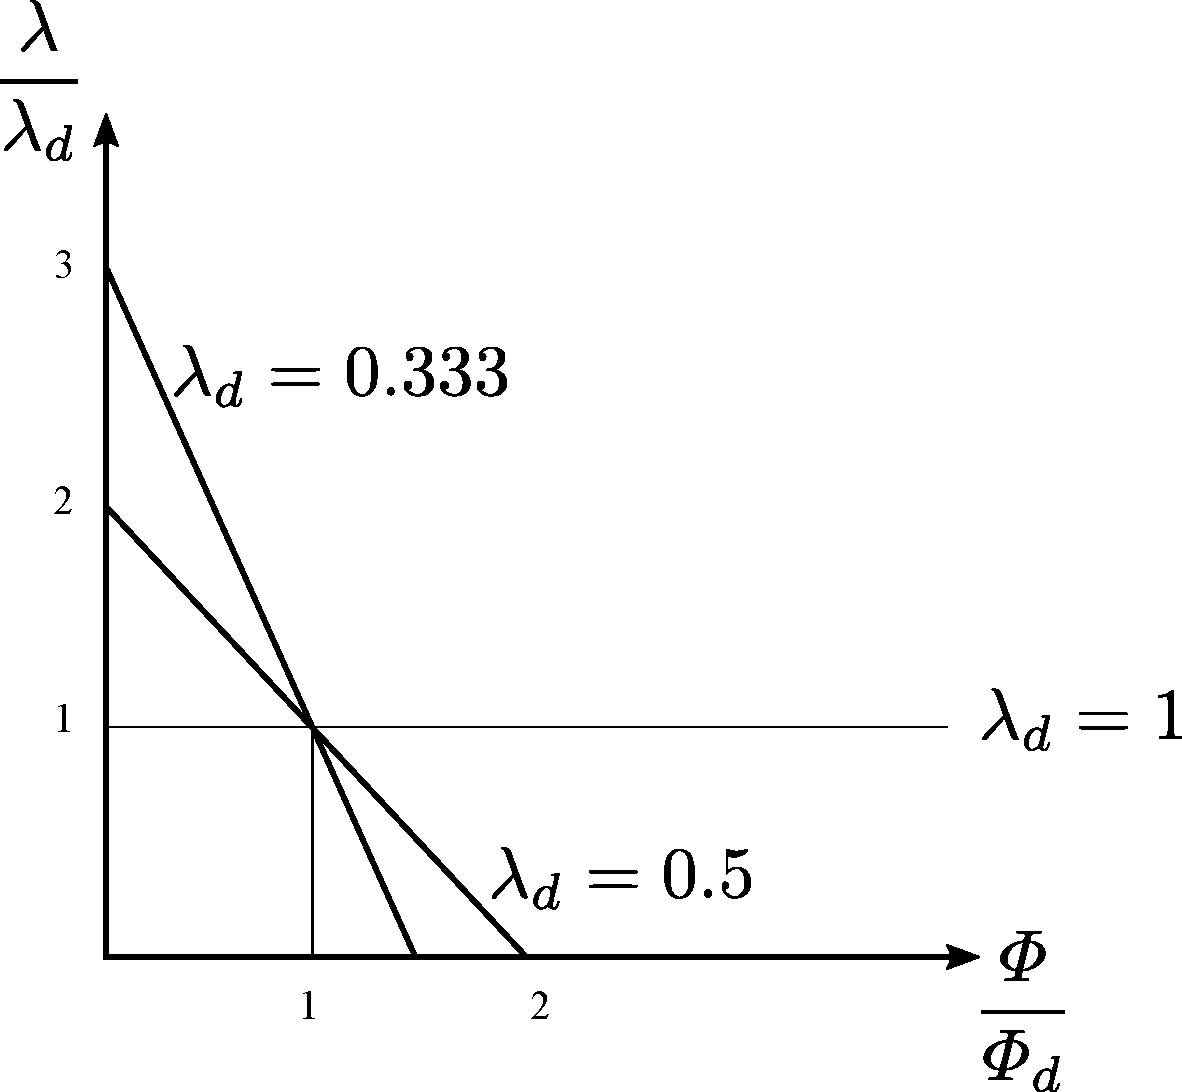
\includegraphics[width=.9\linewidth]{fig/LambdaPhiChart.pdf}
  \captionof{figure}{}
  \label{fig:LambdaPhiChart}
\end{minipage}%
\begin{minipage}{.5\textwidth}
  \centering
  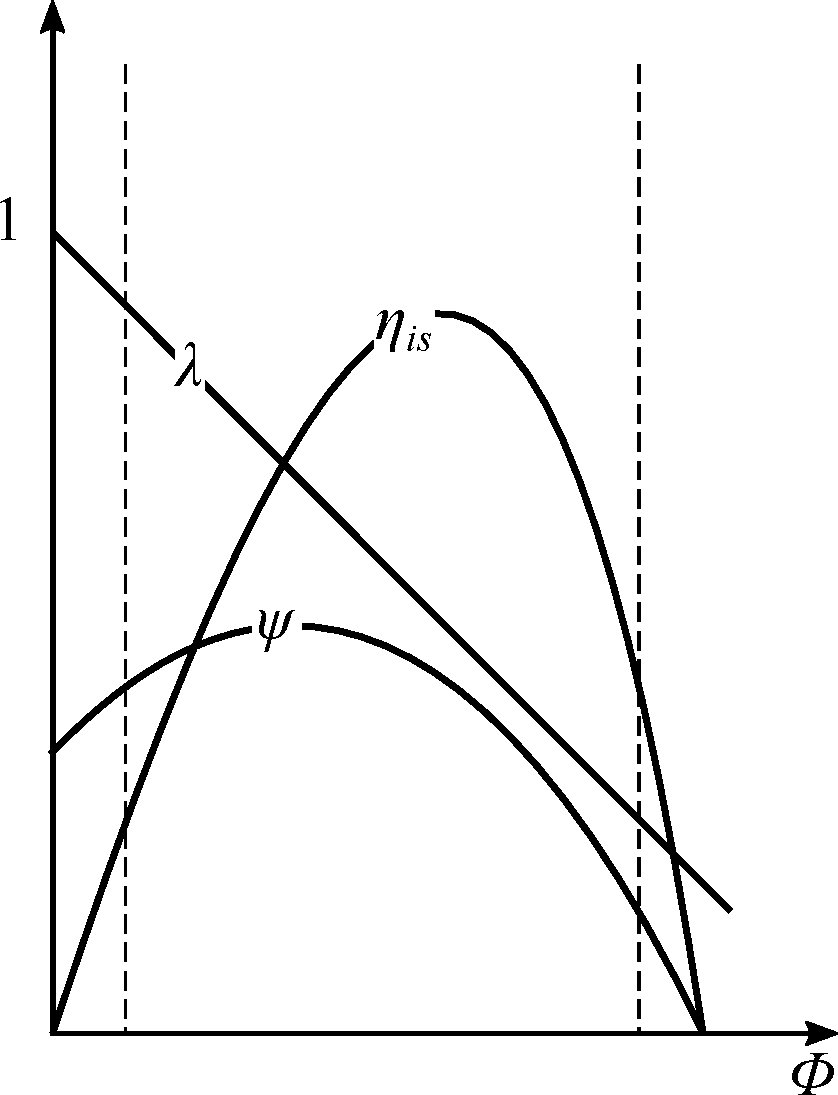
\includegraphics[width=.9\linewidth]{fig/CarattReal.pdf}
  \captionof{figure}{}
  \label{fig:CarattReal}
\end{minipage}
\end{figure}
\\Generalmente in un compressore infatti, la pressione di output è definita mentre la portata è regolata; con $\lambda_d = 1$ si otterrebbe una macchina perfetta: il rapporto di compressione si riuscirebbe sempre a mantenere e basterebbe regolare la portata per ottenere la pressione voluta. Purtroppo non è così perché le palettature non si comportano in modo ideale, si hanno separazioni di vena, inspessimenti di strato limite, ecc. Dal punto di vista realistico si riesce ad ottenere $0.3<\lambda_d<0.4$.

Come mostrato in figura \ref{fig:CarattReal} si otterrà un comportamento non ideale evidenziato dalla curva della caratteristica reale $\psi$; essa non avrà andamento rettilineo e quindi un campo di utilizzo limitato che esclude sia portate basse che portate alte. La caratteristica reale $\psi$ si ottiene moltiplicando la caratteristica ideale per il rendimento:
\begin{equation}
\psi = \frac{\Delta h_{0is}}{u^2} = \lambda \cdot \eta_{is} \;\;\;\; \text{con}\; \Delta h_{0is} = h_{30is} - h_{10}
\end{equation}

Non è ancora stato detto nulla riguardo la forma della pala in funzione del grado di reazione definito come il rapporto tra il salto entalpico elaborato tra parte rotorica e statorica:
\begin{align*}
R = \frac{h_2 - h_1}{h_3-h_1} 
\end{align*}
Sapendo che
\begin{align*}
\begin{rcases*}
c_{u2} = u - w_{u2}\\
c_{u1} = u - w_{u1}
\end{rcases*}
\;\;\;\; \rightarrow \;\;\;\; c_{u2} - c_{u1} = w_{u1} - w_{u2} 
\end{align*}
si sviluppa l'espressione del grado di reazione della macchina applicando la conservazione della rotalpia al numeratore e l'espressione del lavoro euleriano al denominatore:
\begin{align*}
R = \frac{w_1^2 - w_2^2}{2 u (c_{u2} - c_{u1})} &= \frac{(w_{u1} + w_{u2})\cancel{(w_{u1}-w_{u2})}}{2 u \cancel{(c_{u2} - c_{u1})}} =\\
&= \frac{w_{u1} + w_{u2}}{2u} = \\
&= \frac{c_m \left(\tan \beta_1 + \tan \beta_2 \right)}{2 u}
\end{align*}
Definendo poi:
	\begin{align*}
	\tan \beta_{\infty} = \frac{\tan \beta_1 + \tan \beta_2}{2} \;\;\;\;\;\;\;\; \Phi = \frac{c_m}{u}
	\end{align*}
si ottiene
\begin{equation}
\boxed{R = \Phi \tan \beta_{\infty} = \frac{w_{u \infty}}{u}}
\end{equation}
Lo stesso risultato poteva essere raggiunto nel seguente modo:
\begin{align*}
	w_{u1} = u - c_{u1} \;\;\;\; \rightarrow \;\;\;\; R =\frac{(u-c_{u1}+w_{u2})\cancel{(w_{u1}-w_{u2})}}{2 u \cancel{(c_{u2} - c_{u1})}}=\frac{u-c_{u1}+w_{u2}}{2u}
\end{align*}
\begin{equation}
R = \frac{1}{2} + \frac{\tan \beta_2 - \tan \alpha_1}{2} \cdot \Phi \simeq \frac{1}{2} + cost \cdot \Phi
\end{equation}
Quello che è importante notare è che il grado di reazione dipende tramite una costante dalla cifra di portata e che:
\begin{align*}
R = 0.5 \;\;\;\; \to \;\;\;\; \beta_2 = \alpha_1
\end{align*}
ossia che la palettatura sarà simmetrica se $R=0.5$.

Per rappresentare lo stadio al variare del grado di reazione si definiscono i triangoli di velocità (figura \ref{fig:StadioRipetuto}).
\begin{figure}
\centering
  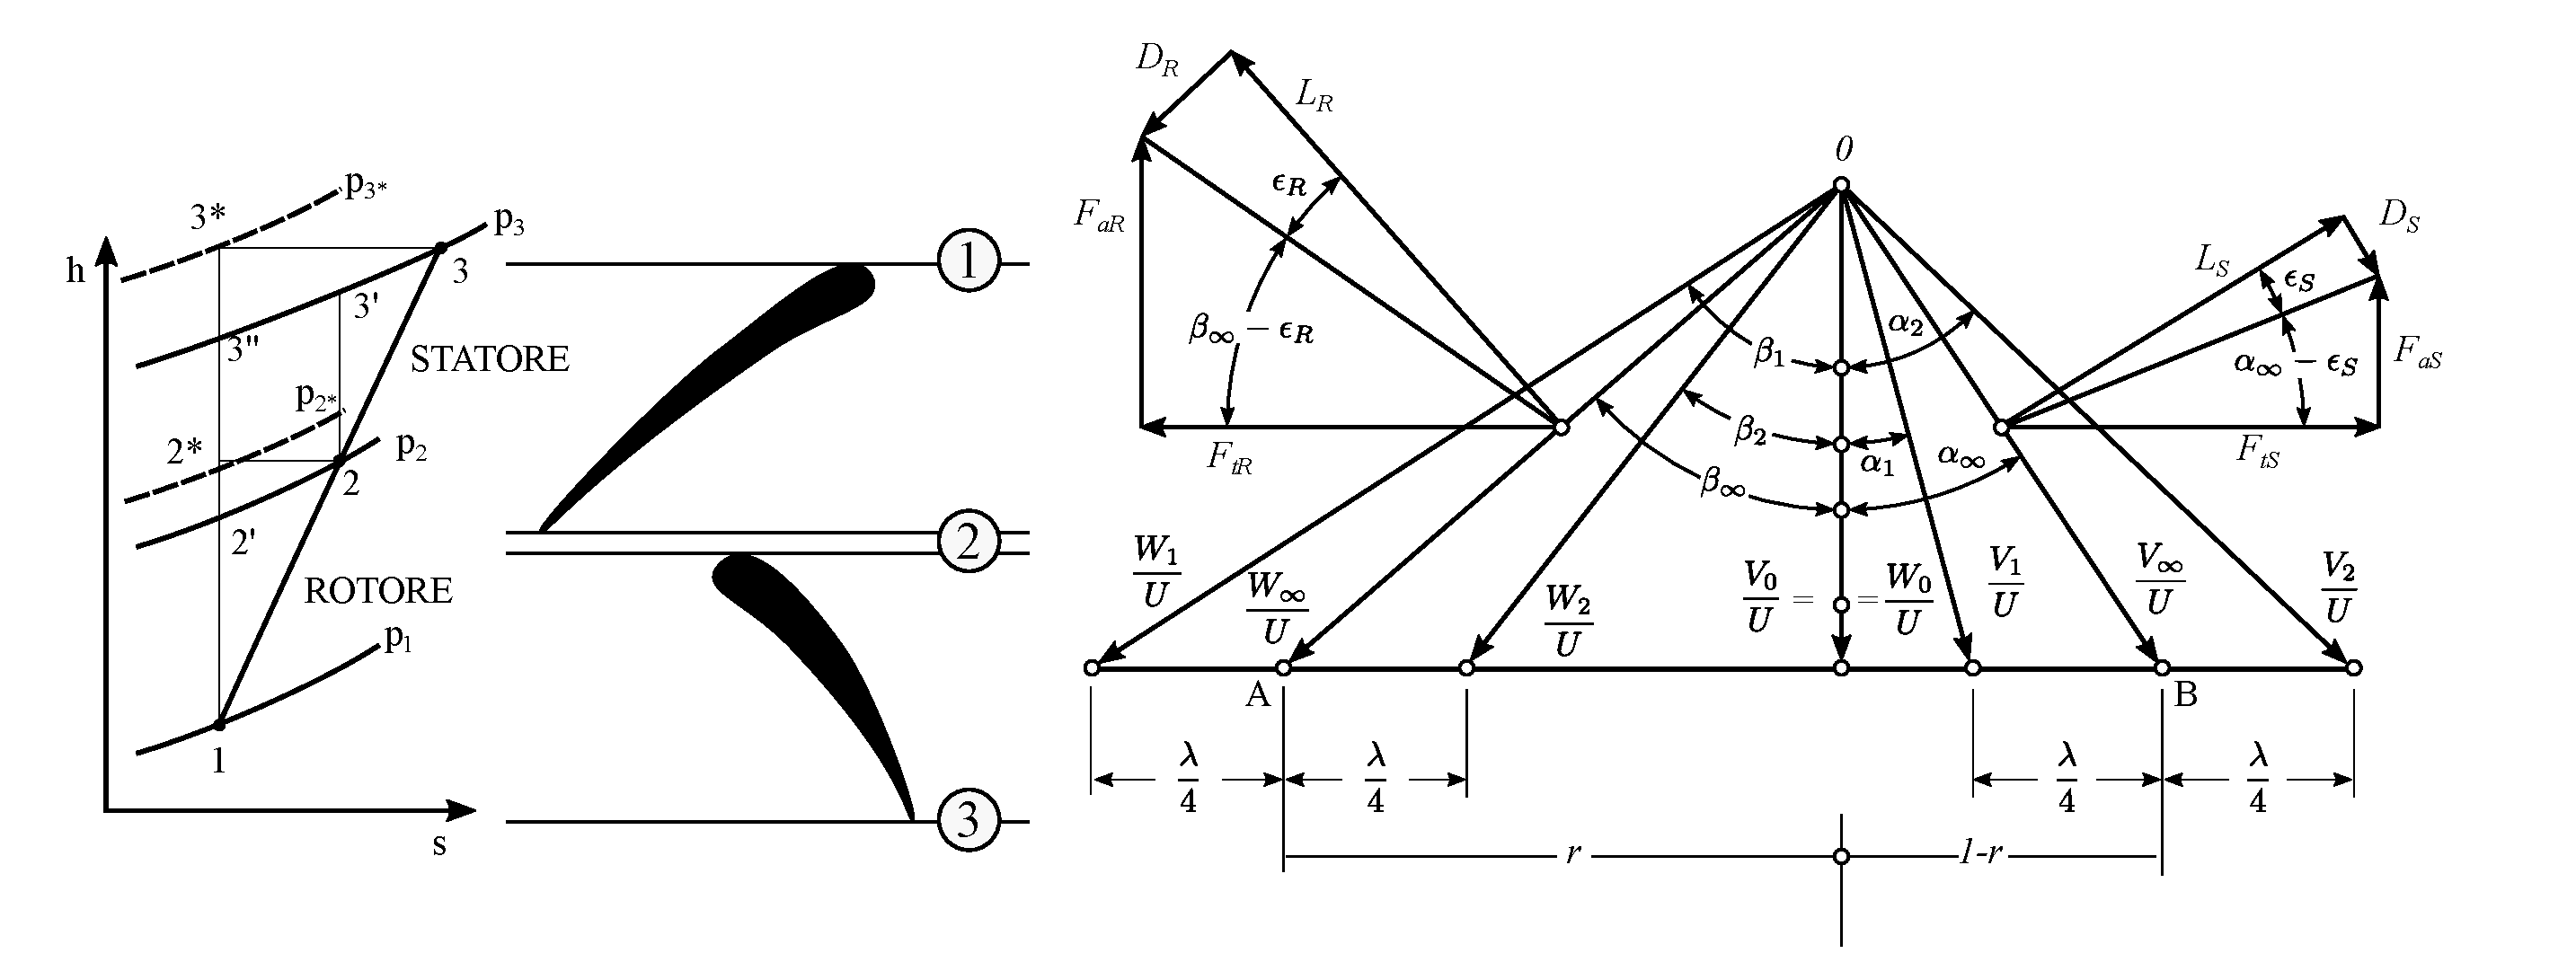
\includegraphics[width=\textwidth]{fig/StadioRipetuto.pdf}
\caption{}
\label{fig:StadioRipetuto}
\end{figure}
Facendo riferimento alla figura si può scrivere:
\begin{align*}
\Phi \cdot \tan \beta_{\infty} = R
\end{align*}
\begin{equation}\label{eq:lambda}
\lambda = \cfrac{\Delta h_0}{\cfrac{u^2}{2}} = \cfrac{u \Delta c_u}{\cfrac{u^2}{2}} = \cfrac{2 \Delta c_u}{u} = \cfrac{2 \Delta w_u}{u} \;\;\;\; \Rightarrow \;\;\;\; \frac{\Delta c_u}{u} = \frac{\Delta w_u}{u} = \frac{\lambda}{2}
\end{equation}
Qualora si operi un cambio di portata, gli unici angoli che si conservano sono $\beta_2$ e $\alpha_1$; la cifra di flusso passa dalle condizioni generiche $\Phi$ alle condizioni di design $\Phi_d$ come si vede in figura \ref{fig:CondFuoriProg}.
\begin{figure}
\centering
  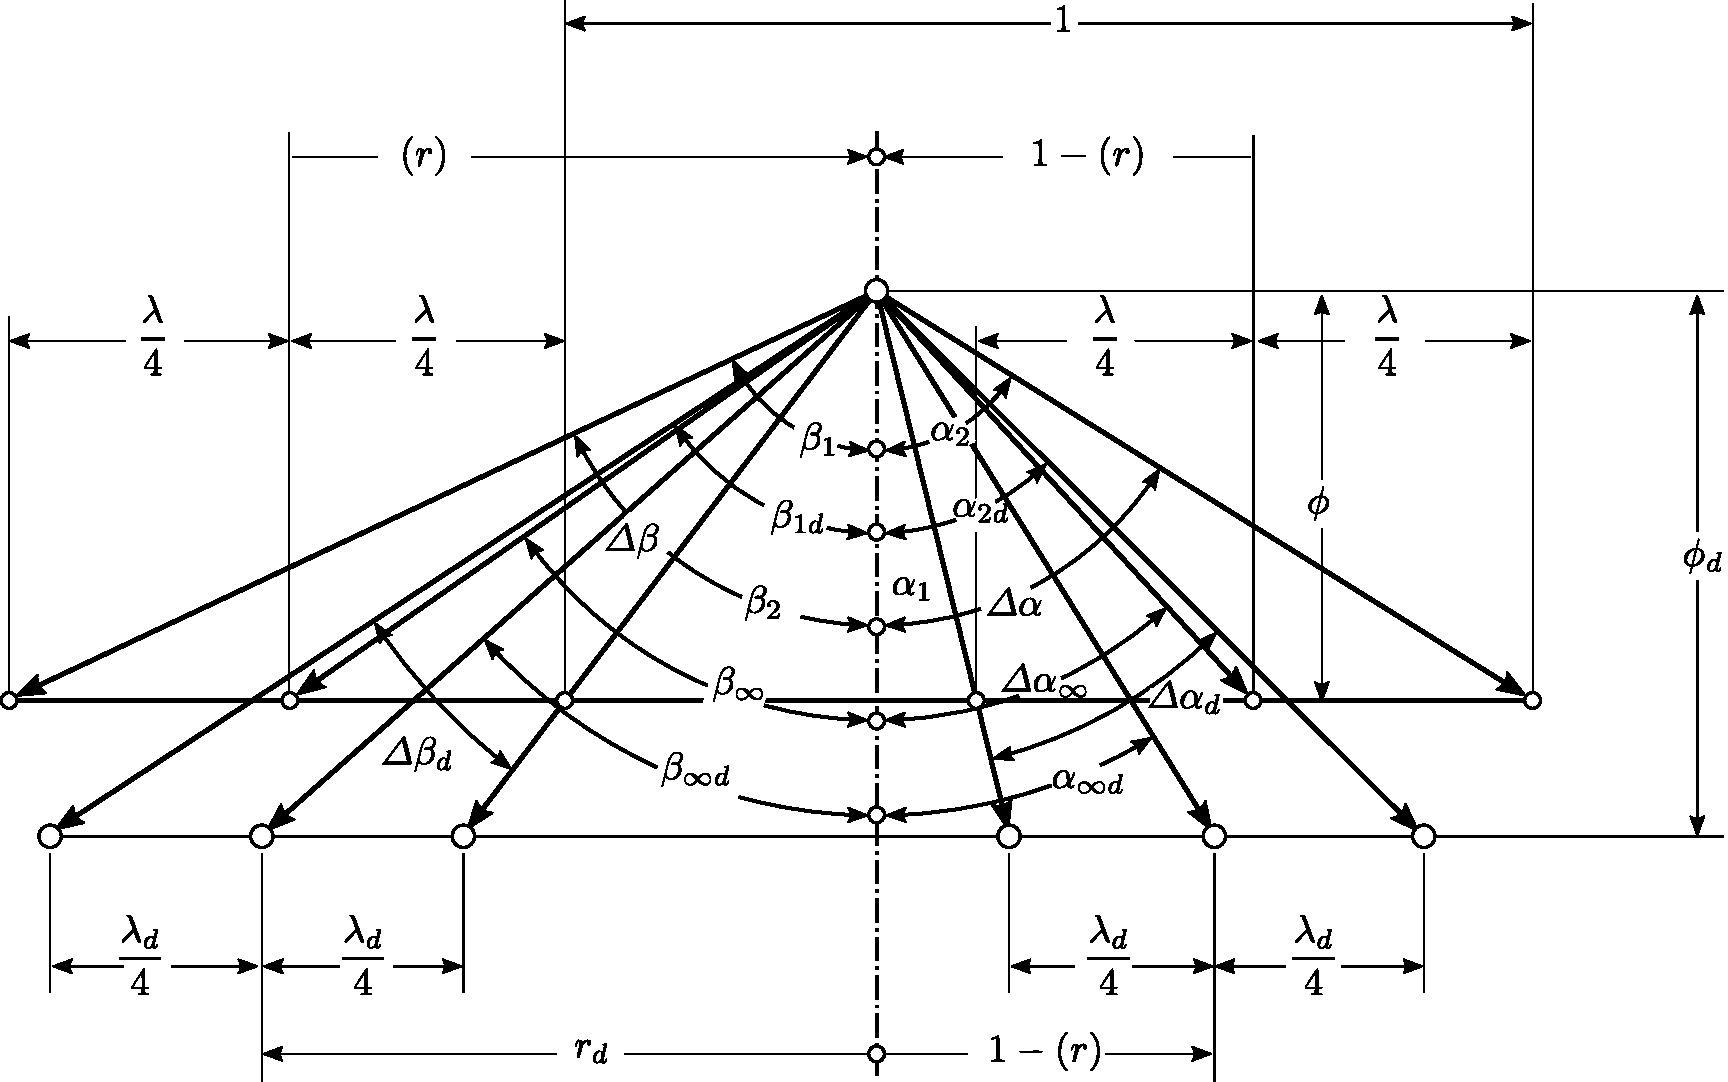
\includegraphics[width=\textwidth]{fig/CondFuoriProg.pdf}
\caption{}
\label{fig:CondFuoriProg}
\end{figure}

Si classificano alcune condizioni notevoli riportate in figura \ref{fig:ComprAssTab}:
\begin{figure}
\centering
  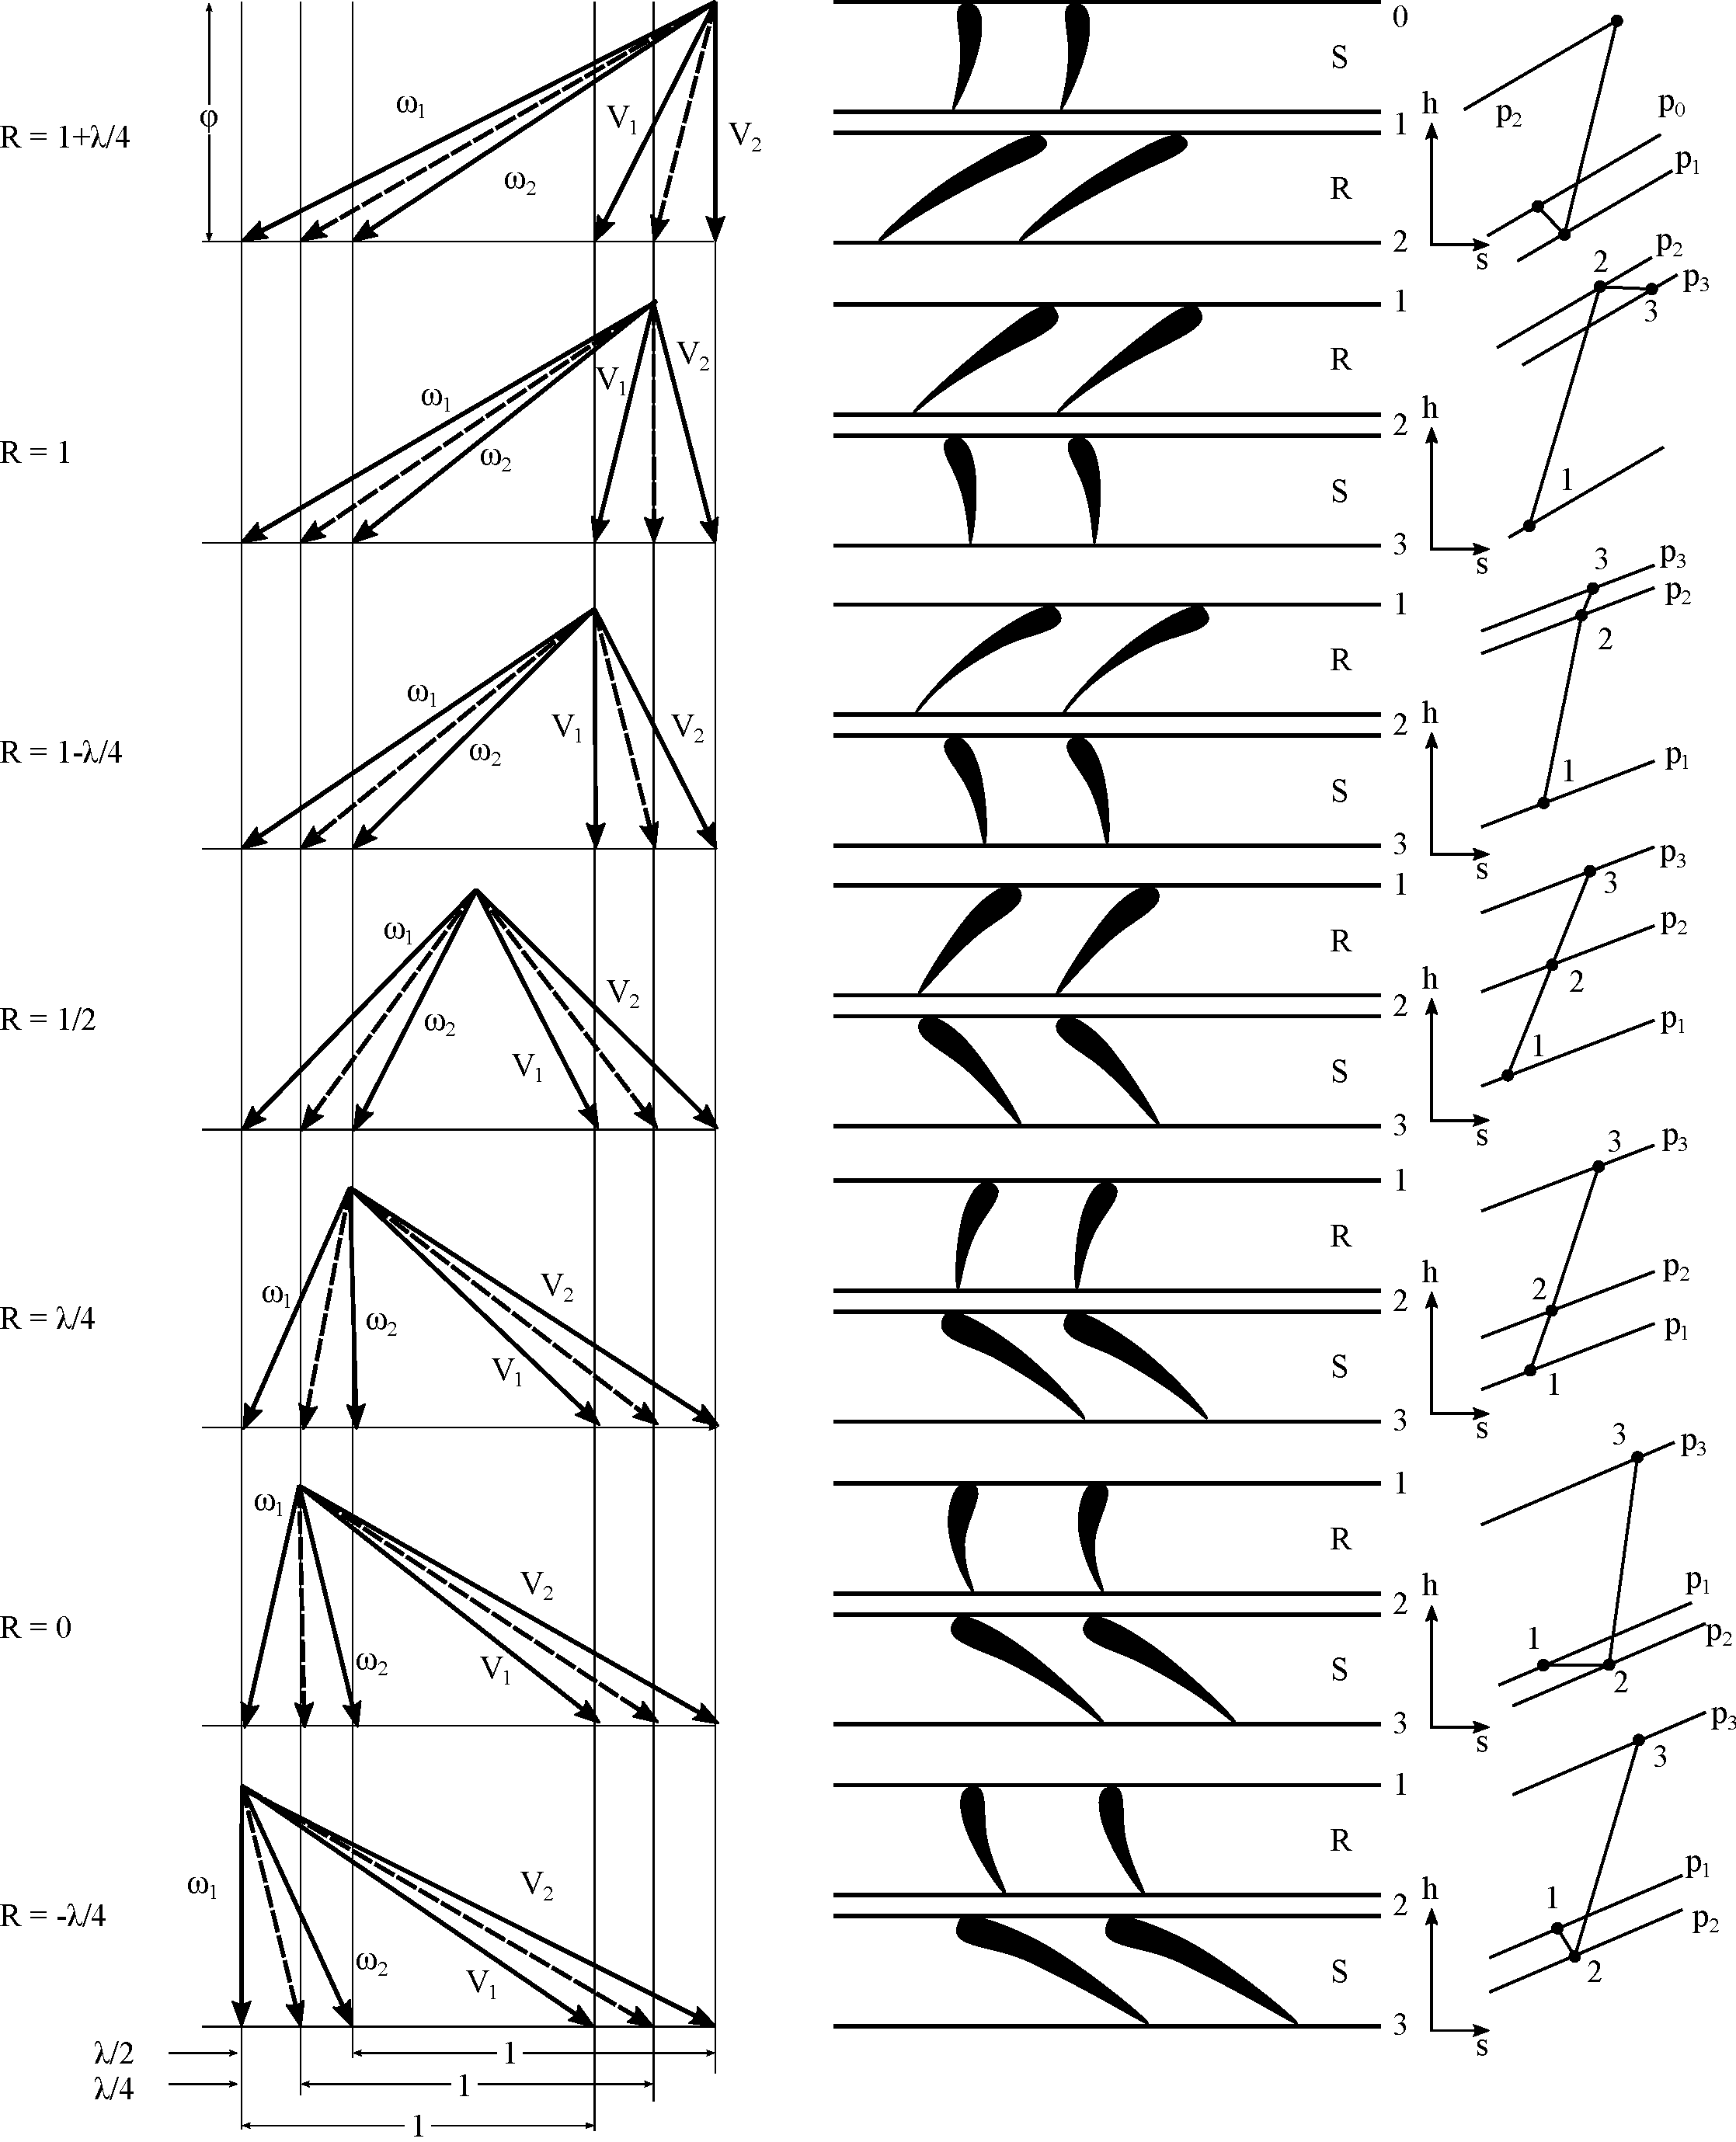
\includegraphics[width=1.2\textwidth]{fig/ComprAssTab.pdf}
\caption{}
\label{fig:ComprAssTab}
\end{figure}
\begin{itemize}
	\item il primo caso con $R = 1 + \lambda /4$ è particolare in quanto si ha grado di reazione maggiore di uno e infatti lo statore precede il rotore. In uscita sarà presente una velocità puramente assiale;

	\item con $R = 1/2$ le velocità assolute in ingresso e uscita sono simmetriche;

	\item con $R = 1 - \lambda/4$ la velocità assoluta è puramente assiale, mentre quella allo scarico non lo è;

	\item sono poi rappresentate le geometrie per gradi di reazione sempre più ridotti. 
\end{itemize}

La soluzione $R = 1/2$ è la più diffusa e utilizzata eccetto per il primo e l'ultimo stadio in cui si vogliono distribuzioni di velocità particolari (si usano rispettivamente $R = 1 - \lambda /4$ e $R = 1 + \lambda /4$). Questa configurazione viene preferita in quanto si avranno profili uguali ma specchiati e l'incremento di pressione (da $p_1$ a $p_3$) è diviso equamente in due parti uguali tra la parte statorica e la parte rotorica. 

\section{Termodinamica}
Si calcola il rendimento al variare della portata e del grado di reazione. Si definisce il rendimento isoentropico:
\begin{align*}
\eta_{is} = \frac{\Delta h_{is}}{\Delta h_0}
\end{align*}
Dal primo principio della termodinamica:
\begin{align*}
T ds = dh - \frac{dp}{\rho}
\end{align*}
ma
\begin{align*}
ds = 0 \;\;\;\; \rightarrow \;\;\;\; dh = \frac{dp}{\rho}
\end{align*}
Si ottiene, ricordando la definizione \ref{eq:lambda} di $\lambda$, quindi:
\begin{equation}\label{eq:etadp}
\eta_{is} = \frac{\Delta p}{\rho \cdot \Delta h_0} = \cfrac{\Delta p}{\rho \cdot \cfrac{\lambda}{2} u^2}
\end{equation}
Considerando i triangoli di velocità (figura \ref{fig:StadioRipetuto}), l'incremento di pressione totale si può ulteriormente sviluppare come somma di incremento di pressione sviluppato nel rotore e nello statore:
\begin{equation}
\Delta p = \Delta p_R + \Delta p_S = \frac{F_{aR}}{s_R} + \frac{F_{aS}}{s_S} = \frac{F_{tR} \cdot \tan(\beta_{\infty} - \varepsilon_R)}{s_R} + \frac{F_{tS} \cdot \tan(\alpha_{\infty} - \varepsilon_S)}{s_S}
\label{eq:deltap}
\end{equation}
con $\varepsilon_S$ e $\varepsilon_R$ indici di efficienza del profilo e $s_R$ e $s_S$ i passi\footnote{Per quanto riguarda i pedici "S" sta per statore, "R" sta per rotore.}.\\
Si può fare qualche assunzione: i profili hanno drag molto più piccolo del lift quindi:
\begin{align*}
\tan \varepsilon_R \simeq \varepsilon_R = \frac{D_R}{L_R} \;\;\;\;\;\;\;\; \tan \varepsilon_S \simeq \varepsilon_S = \frac{D_S}{L_S}
\end{align*}
Utilizzando le componenti di forza del triangolo di velocità per rotore e statore, e ricordando la definizione di $\Phi$, si ottiene:
\begin{align*}
F_{tR} = \dot{m} \cdot \Delta w_u = \overbrace{s_R \cdot \rho \cdot c_m}^\text{$ \dot{m} $} \cdot \overbrace{\lambda \cdot u \cdot \frac{1}{2}}^\text{$\Delta w_u$}=  s_R \cdot \rho \cdot \lambda \cdot \Phi \cdot u^2 \cdot \frac{1}{2}
\end{align*}
\begin{align*}
F_{tS} = \dot{m} \cdot \Delta c_m = s_S \cdot \rho \cdot c_m \cdot \lambda \cdot u \cdot \frac{1}{2} =s_S \cdot \rho \cdot \lambda \cdot \Phi \cdot u^2 \cdot \frac{1}{2}
\end{align*}
Andando a sostituire le due forze nell'equazione \ref{eq:deltap}:
\begin{align*}
\Delta p = \frac{1}{2} \rho \lambda u^2 \big[\Phi \tan \left( \beta_{\infty} - \varepsilon_R \right) + \Phi \tan \left( \alpha_{\infty} - \varepsilon_S \right) \big]
\end{align*}
e ricordando le relazioni
\begin{align*}
R = \Phi \tan \beta_{\infty} \;\;\;\;\;\;\;\;\;\;\; 1 - R = \Phi \tan \alpha_{\infty} 
\end{align*}
\begin{align*}
\tan ( \beta_{\infty} - \varepsilon_R ) = \frac{\tan \beta_{\infty} - \tan \varepsilon_R}{1 + \tan \beta_{\infty} \tan \varepsilon_R} \simeq \frac{\tan \beta_{\infty} - \varepsilon_R}{1 + \tan \beta_{\infty} \varepsilon_R}= \frac{R - \varepsilon_R \Phi}{\Phi + \varepsilon_R R}
\end{align*}
\begin{align*}
\tan (\alpha_{\infty} - \varepsilon_S) \simeq \frac{\tan \alpha_{\infty} - \varepsilon_S}{1 + \tan \alpha_{\infty} \cdot \epsilon_S} = \frac{1 - R - \varepsilon_S \Phi}{\Phi + \varepsilon_S (1-R)}
\end{align*}
Si ottiene infine la relazione del salto di pressione in funzione del grado di reazione e di $\lambda$:
\begin{equation}
\Delta p = \frac{1}{2} \rho \lambda u^2 \Bigg[ \frac{R - \varepsilon_R \Phi}{\Phi + \varepsilon_R R} + \frac{1 - R - \varepsilon_S \Phi}{\Phi + \varepsilon_S (1-R)} \Bigg]
\end{equation}
Il rendimento isoentropico, ricordando l'equazione \ref{eq:etadp}, diviene:
\begin{equation}
\boxed{ \eta_{is} = \Bigg[ \frac{R - \varepsilon_R \Phi}{\Phi + \varepsilon_R R} + \frac{1 - R - \varepsilon_S \Phi}{\Phi + \varepsilon_S (1-R)} \Bigg] }
\end{equation}
Si introduce una semplificazione sugli indici di efficienza e si cerca il coefficiente di reazione ottimale:
\begin{align*}
\varepsilon_S \simeq \varepsilon_R = cost = \varepsilon
\end{align*}
\begin{align*}
\frac{d \eta_{is}}{dR} = 0 \;\;\;\; \text{se}  \;\;\;\; R_{opt} = 0.5 \mbox{ per } \forall \Phi
\end{align*}
Il rendimento con questo valore di R vale:
\begin{equation}
\eta_{|R= 0.5} = 2 \Phi \cdot \frac{1- 2 \varepsilon \Phi}{\varepsilon + 2 \Phi}
\end{equation}
Il rendimento del compressore è migliorato alla diminuzione di $\varepsilon$. Questa relazione lega il rendimento alla portata e all'efficienza del profilo; per il progetto di un compressore si inizierà quindi dallo studio del singolo profilo visto che le sue prestazioni hanno influenza sul rendimento totale.\\
Si determina ora il valore di $\Phi$ che rende massimo il rendimento ottimale:
\begin{align*}
\frac{d\eta_{|R=0.5}}{d \Phi} = 0 \;\;\;\; \text{se} \;\;\;\; \Phi_{opt} = \frac{1}{2} \left( \sqrt{1 + \varepsilon^2} - \varepsilon \right) \simeq \frac{1 - \varepsilon}{2}
\end{align*}
\begin{equation}
\eta_{max} = 1 + 2 \varepsilon^2 - 2 \varepsilon \sqrt{1 + \varepsilon^2} \simeq 1 - 2 \varepsilon \left( 1 - \varepsilon \right)
\end{equation}
\begin{figure}
\centering
  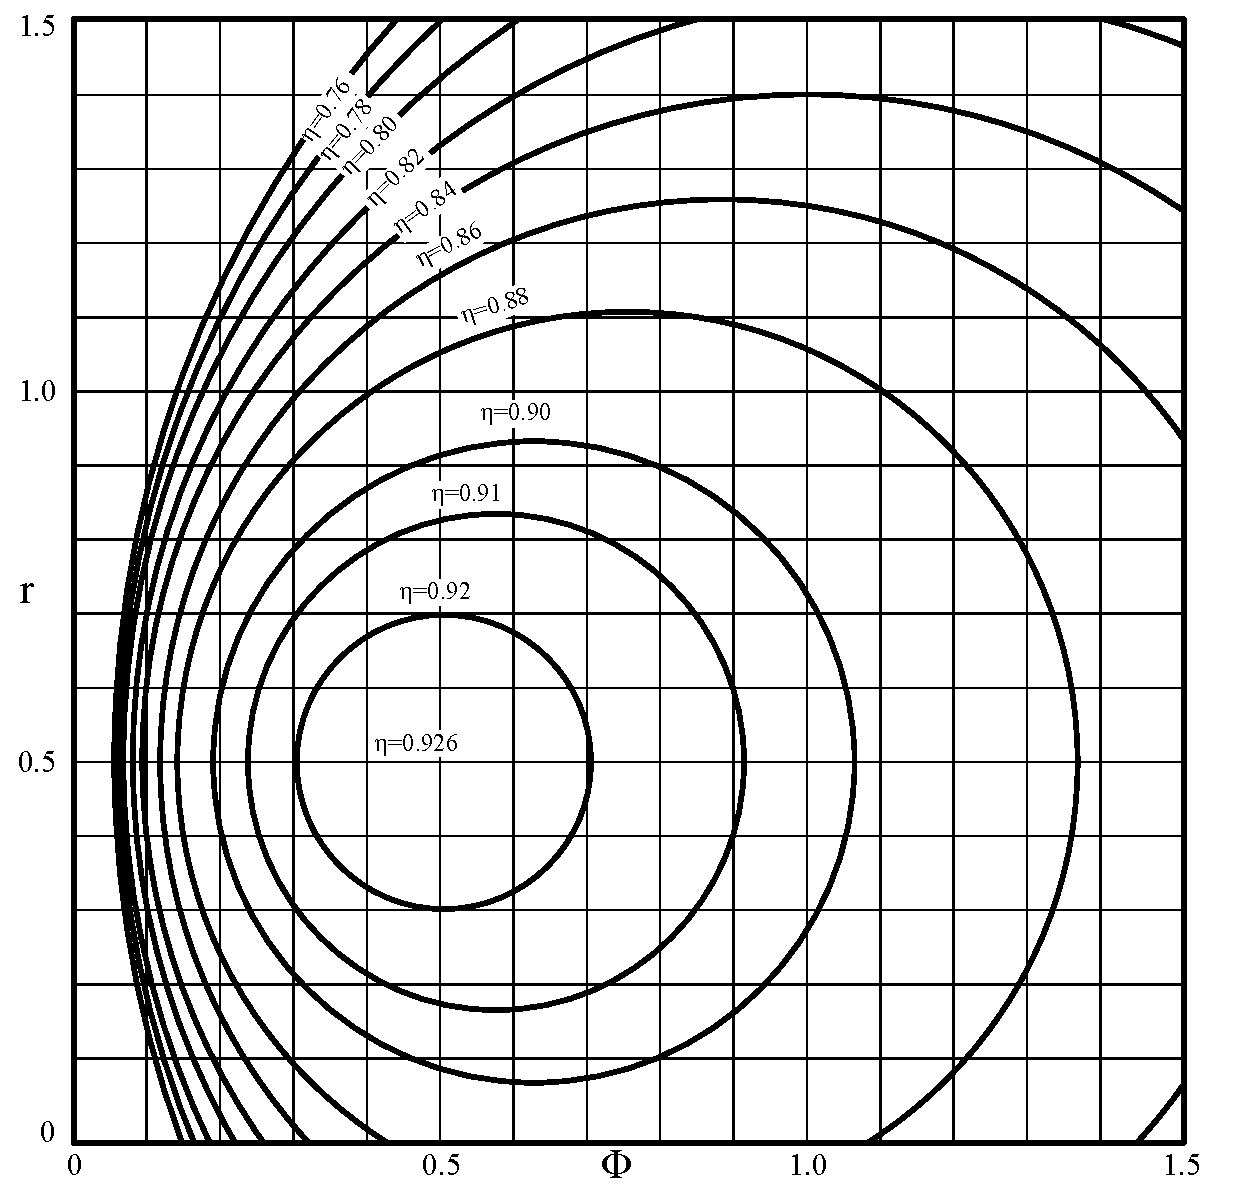
\includegraphics[width=\textwidth]{fig/IsoRendCompAss.pdf}
\caption{Curve isorendimento di uno stadio assiale in funzione del grado di reazione e coefficiente di portata per efficienza del profilo $\epsilon=0.04$}
\label{}
\end{figure}

\section{Progettazione della schiera}
Sono presenti molteplici correlazioni per progettare una macchina assiale. Si analizzeranno un filone di correlazioni datate ma che non hanno perso di validità. Anche nella progettazione di una nuova macchina è utile partire da un predimensionamento per poi andare a raffinare lo studio con strumenti moderni. Queste correlazioni verranno quindi usate come passo preliminare.\\
\'E possibile fare le seguenti riflessioni:
\begin{itemize}
\item la deflessione imposta alla corrente è limitata: nell'ordine delle decine di gradi ($20 \div 30$ al massimo $40$);
\item profili sottili a bassa curvatura.
\end{itemize}
Le perdite possono quindi essere suddivise in:
\begin{itemize}
\item perdite di anello: sono dovute all'interazione tra flusso elicoidale che si sviluppa all'interno del compressore e la cassa della macchina. Esse inducono un drag aggiuntivo correlato a quanto più è elevato lo sviluppo radiale della pala. Definito $H$ lo sviluppo radiale e $s$ passo palare, si può scrivere:
\begin{align*}
C_{Da} = 0.02 \cdot \frac{s}{H}
\end{align*}
\item perdite di profilo: sono direttamente correlate al coefficiente $c_D$, saranno quelle in cui si può andare maggiormente a lavorare;
\item perdite per flussi secondari: trattate nel capitolo precedente. Esse sono dipendono dal quadrato del coefficiente di portanza; tanto più la portanza è elevata tanto verrà imposta una deviazione e di conseguenza tanto più è probabile che si instaurino moti secondari.
\begin{align*}
C_{Ds} = 0.018 \cdot c_L^2
\end{align*}
\end{itemize}
\'E possibile andare quindi a scrivere un coefficiente di resistenza complessivo:
\begin{equation}
C_{Dtot} = C_D + C_{Da} + C_{Ds} = C_D + 0.02 \cdot \frac{s}{H} + 0.018 \cdot c_L^2
\label{eq:Cdtot}
\end{equation}
In questo modo si riconducono le perdite all'interno del flusso ad un incremento del coefficiente di resistenza del profilo. In figura \ref{fig:ComprStageLoss} si vede come le varie perdite inficino sull'efficienza della schiera.
\begin{figure}
\centering
  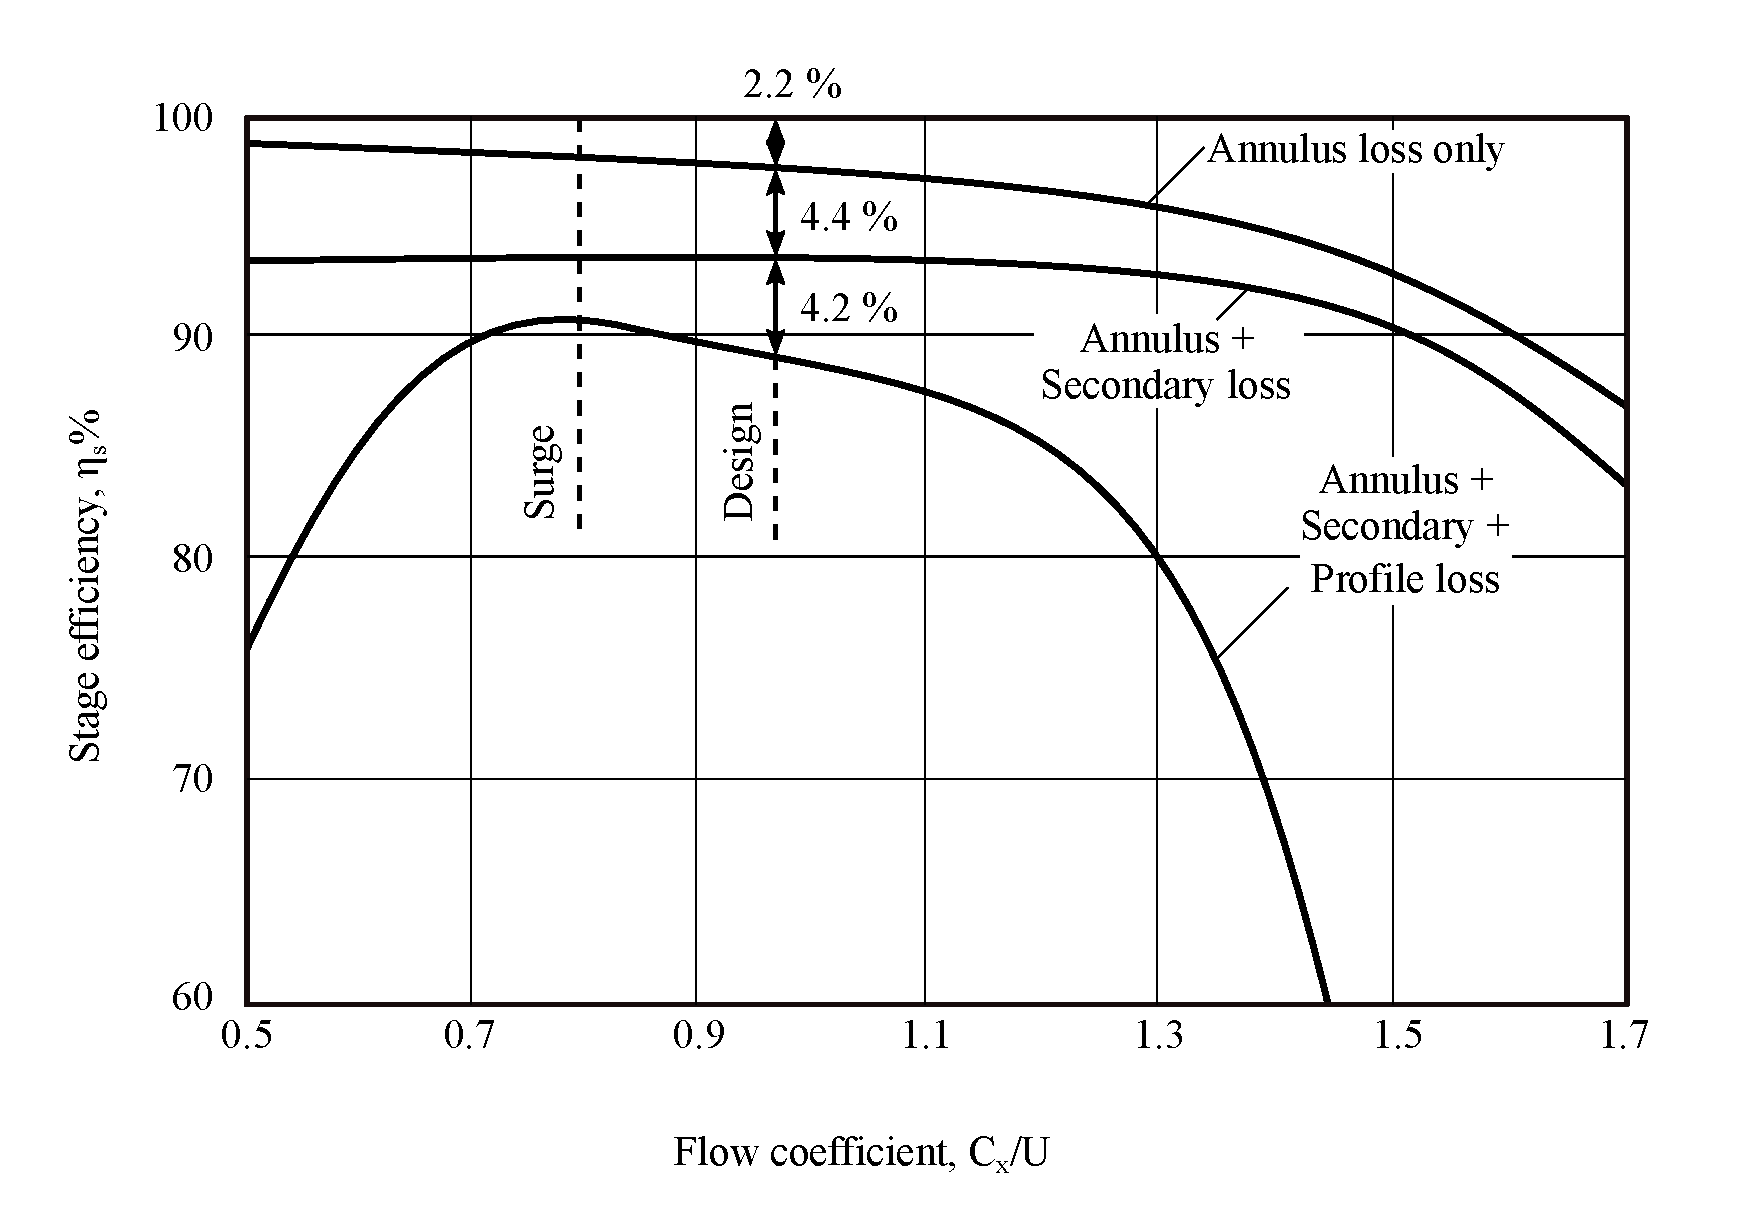
\includegraphics[width=\textwidth]{fig/ComprStageLoss.pdf}
\caption{}
\label{fig:ComprStageLoss}
\end{figure}
\subsection{Correlazioni di Howell}
Si ricordano le nomenclature utilizzate in questo capitolo in figura \ref{fig:SchieraDim}; in particolare è evidenziata la differenza tra angoli geometrici e fluidodinamici.
\begin{figure}
	\centering
	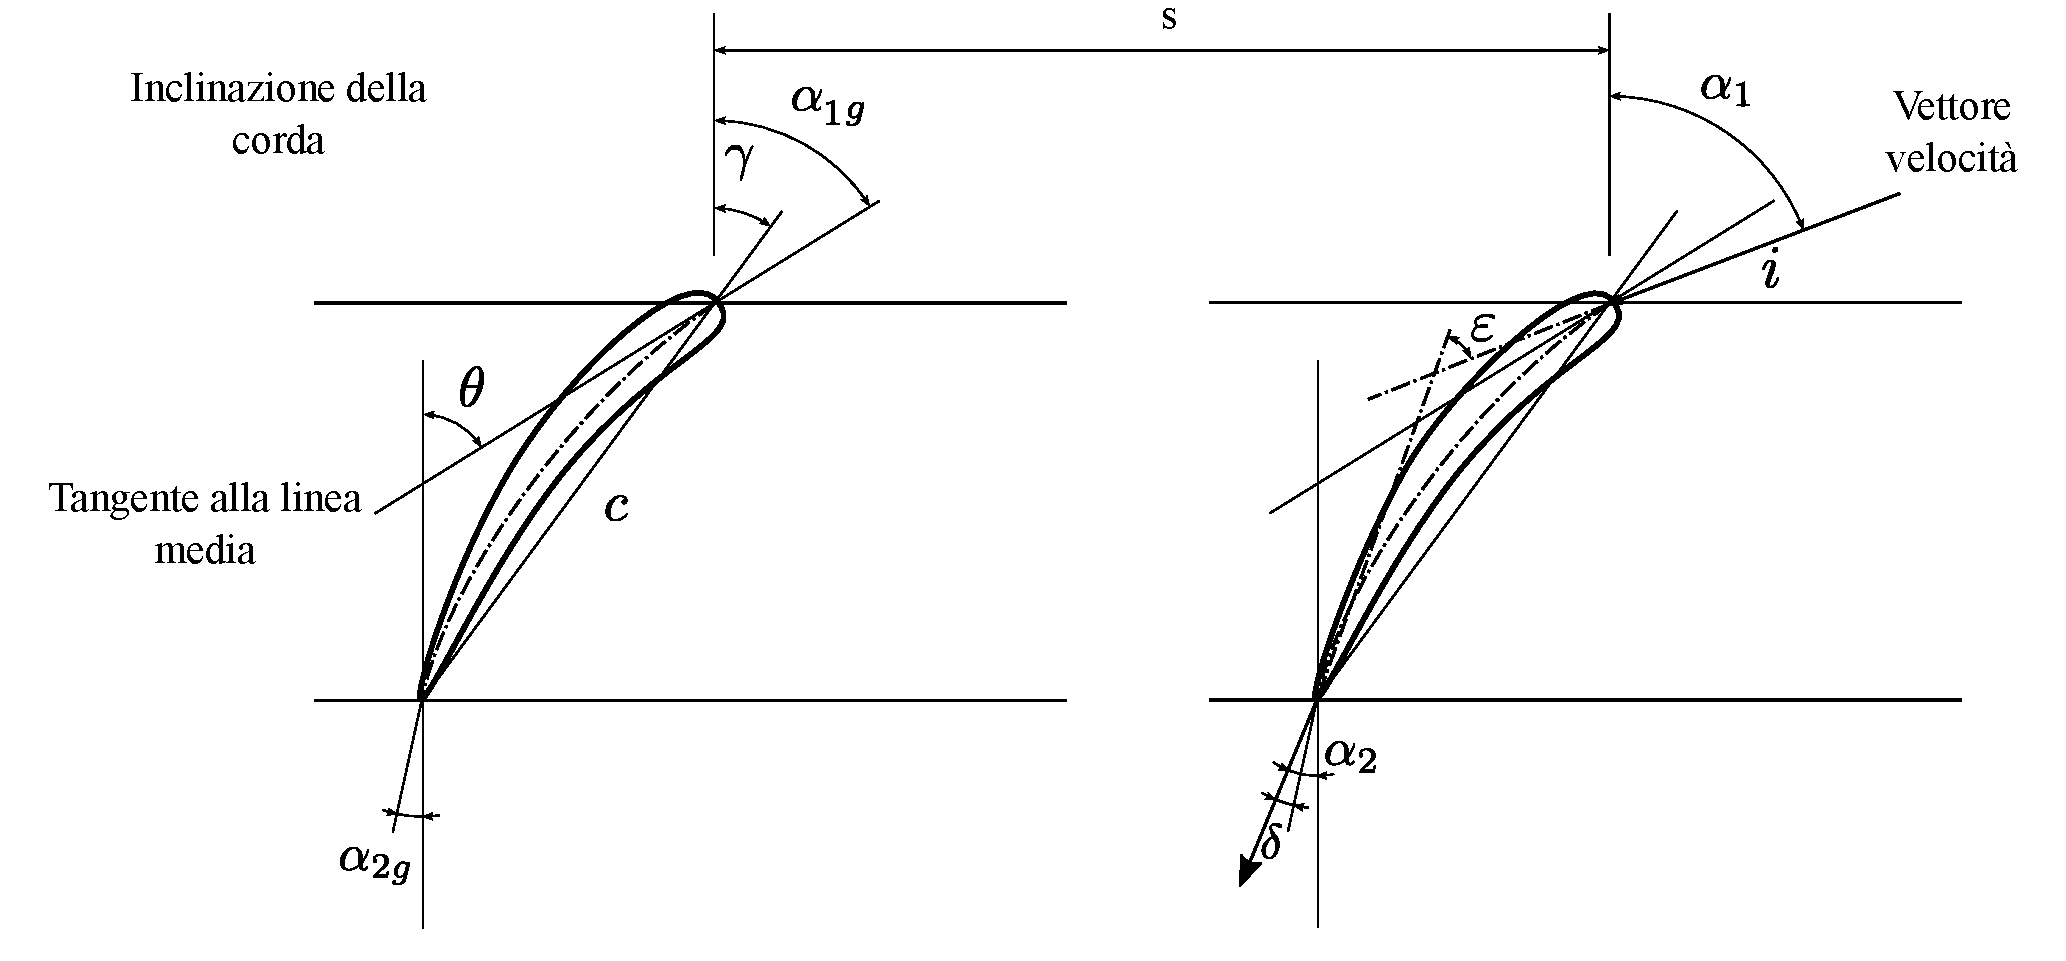
\includegraphics[width=\textwidth]{fig/SchieraDim.pdf}
	\caption{}
	\label{fig:SchieraDim}
\end{figure}

Nella progettazione preliminare fatta utilizzando la correlazione di Howell, si va a cercare la relazione tra gli angoli geometrici in ingresso e in uscita e gli angoli che deve avere il fluido.

La correlazione di Howell dice che la condizione di riferimento, ovvero la deflessione nominale che la corrente subisce nell'attraversamento delle pale $\varepsilon^*$, dipende dalla deviazione di stallo $\varepsilon_s$:
\begin{equation}
\varepsilon^* = 0.8 \cdot \varepsilon_s
\end{equation}
In figura \ref{fig:Howell} è rappresentato l'andamento della deflessione in funzione dell'angolo di incidenza. Come si nota è presente un tratto pressoché lineare seguito da un brusco cambiamento di curvatura dovuto allo stallo. Quest'ultimo è facilmente individuabile e risulta quindi comodo utilizzarlo come punto di riferimento per individuare la deflessione nominale. Come deflessione nominale si utilizzerà quindi un valore che va a minimizzare le perdite, tenendo conto poi dei margini di operabilità.  
\begin{figure}
\centering
  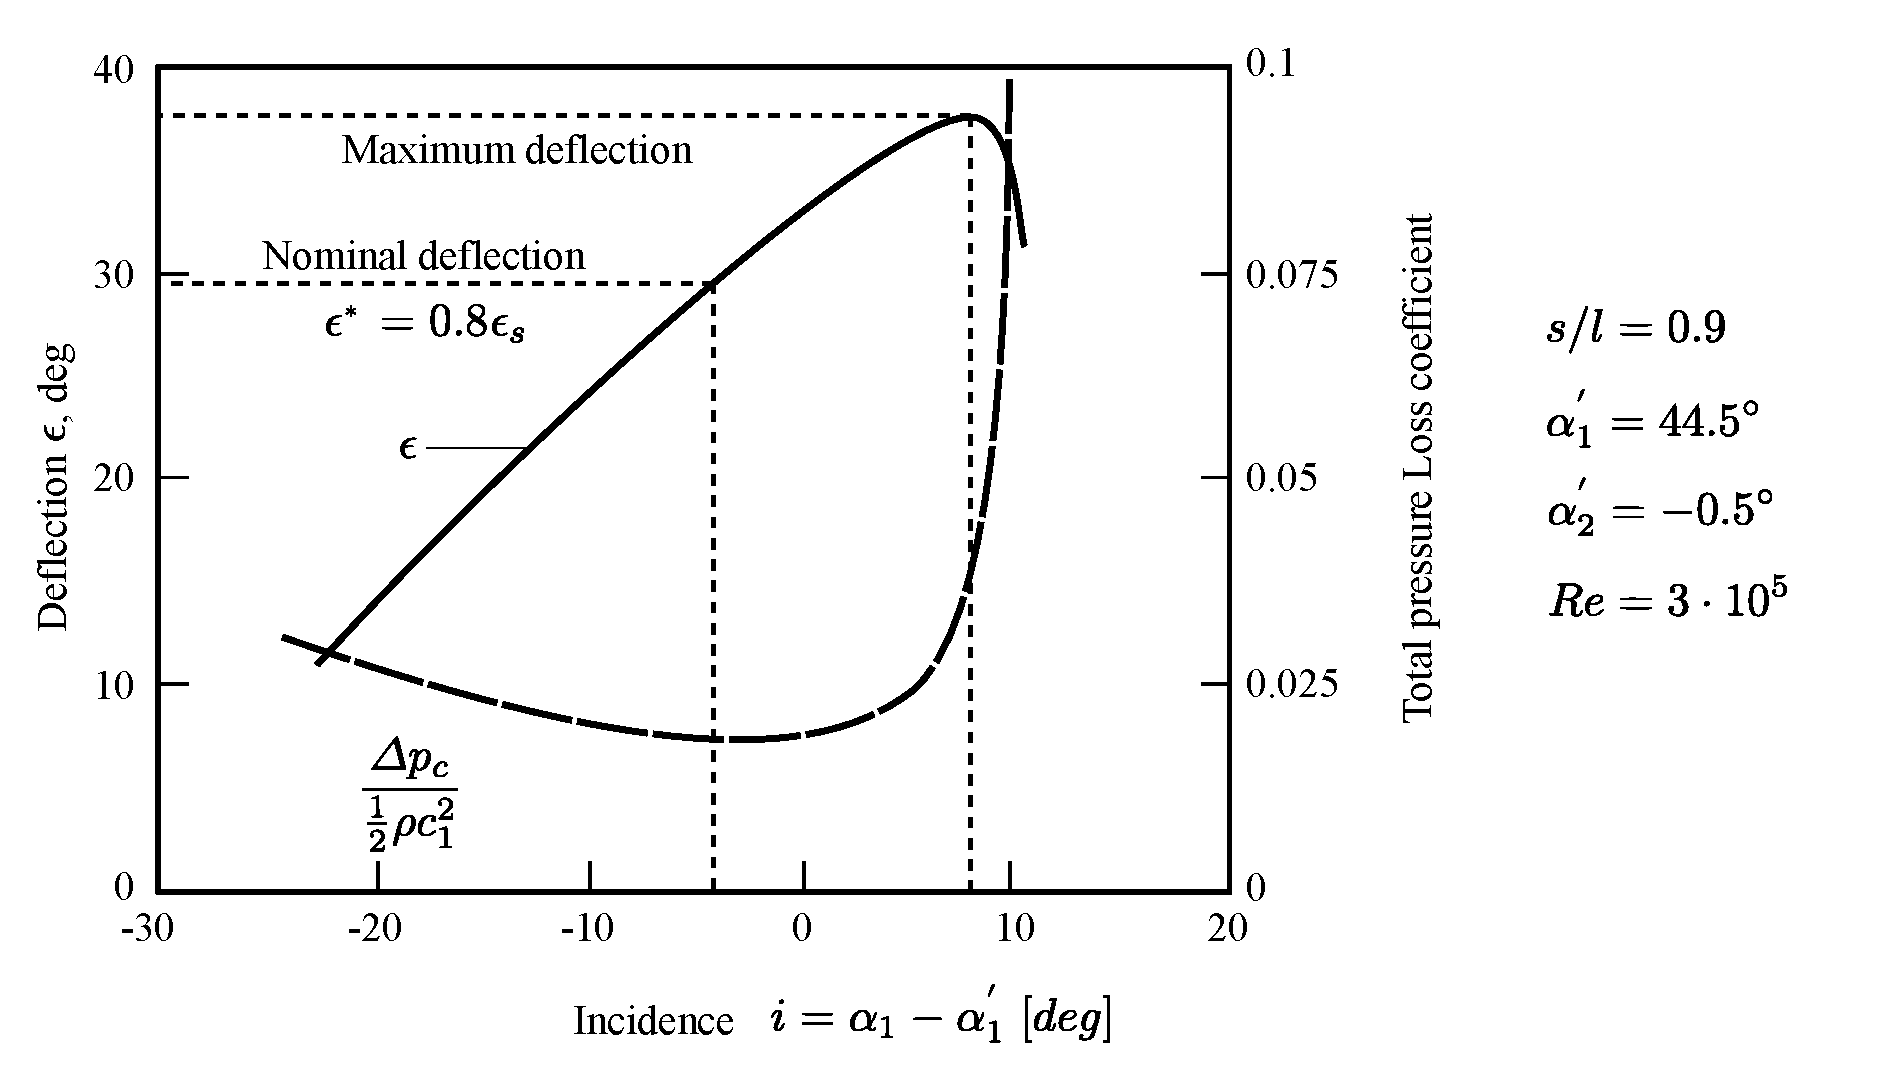
\includegraphics[width=\textwidth]{fig/Howell.pdf}
\caption{}
\label{fig:Howell}
\end{figure}

La prima correlazione di Howell permette di calcolare gli angoli del flusso attesi da una schiera di data solidità ($\epsilon=\epsilon^*$). Questa viene riportata in figura \ref{fig:1CorrHowell} al variare della solidità della schiera. Si nota che a parità di deflessione nominale si avrà una maggiore angolo in uscita per schiere più compatte.
\begin{figure}
	\centering
	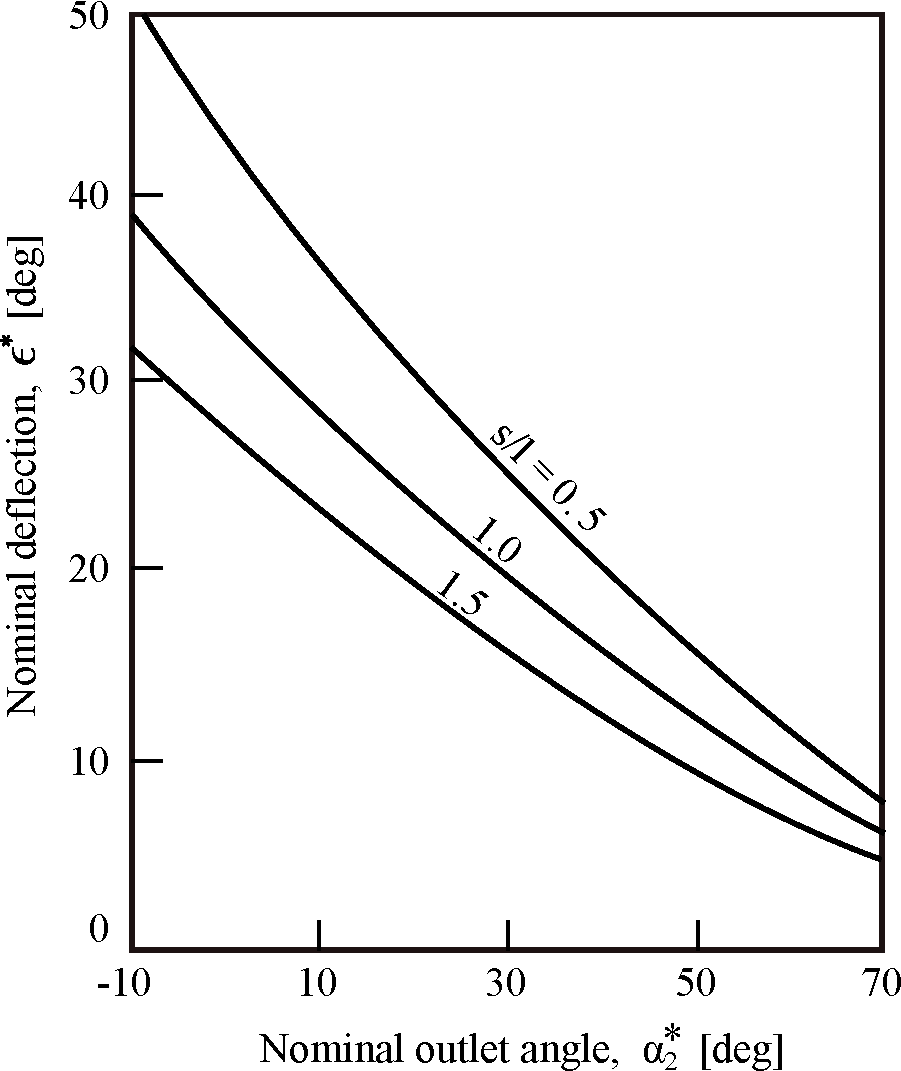
\includegraphics[width=.4\textwidth]{fig/1CorrHowell.pdf}
	\caption{Prima correlazione di Howell, $l$ è la corda del profilo}
	\label{fig:1CorrHowell}
\end{figure}
Se $ 20^{\circ} < \theta < 40^{\circ} $, la relazione della deflessione nominale è indipendente dall'angolo di deflessione geometrica $\theta$:
\begin{align*}
\varepsilon^* = f \bigg( \frac{s}{l}, \alpha_2^*, Re \bigg)
\end{align*}
e se $Re > 3 \cdot 10^5$, la correlazione diventa anche indipendente dal numero di Reynolds:
\begin{align*}
\varepsilon^* = f\bigg(\frac{s}{l}, \alpha_2^*\bigg)
\end{align*}
La deflessione nominale è definita come
\begin{align*}
\varepsilon^* = \alpha_1^* - \alpha_2^*
\end{align*}
e si può scrivere:
\begin{align*}
\boxed{\tan \alpha_1^* - \tan \alpha_2^* = \cfrac{1.55}{1 + 1.5 \cfrac{s}{l}}}
\end{align*}
valida nel range $0^\circ \leq \alpha_2^* \le 40^\circ$.

La seconda correlazione di Howell permette di trovare, noti gli angoli di flusso, i corrispondenti valori degli angoli geometrici della schiera ($\varepsilon = \varepsilon^*$). \'E possibile calcolare il valore della deviazione $\delta$ ossia lo scostamento tra angolo geometrico e angolo effettivo del flusso in uscita:
\begin{align*}
\delta = f \bigg( \theta, forma \; della \; pala, \frac{s}{l}, \gamma \bigg)
\end{align*}
con $\gamma$ angolo di calettamento. Si usa la seguente relazione, nota come legge di Costant:
\begin{align*}
\boxed{\delta^* = m \theta \bigg( \frac{s}{l} \bigg)^n}
\end{align*}
con $n = 1/2$ per schiere di compressore e $n = 1$ per schiere di IGV. Il coefficiente $m$ è funzione della forma della pala, in particolare della sua linea media (queste restano comunque delle correlazioni approssimative visto che derivano da osservazioni sperimentali):
\begin{align*}
m = 0.23 \cdot \bigg( 2 \cdot \frac{a}{l} \bigg)^2 + \frac{\alpha_2^*}{500}
\end{align*}
con $a$ che rappresenta la distanza del punto di massimo incurvamento della linea media rispetto il bordo d'ingresso. 

Con queste correlazioni si riducono i gradi di libertà nella definizione della geometria. Infatti una volta scelti $ \theta$ e $\sigma $, dalla seconda correlazione risulta $ \delta^* $ e dalla prima correlazione si trova $ \varepsilon^* $. In questo modo si definiscono:
\begin{align*}
i^* = \varepsilon^* - \theta + \delta^*
\end{align*}
\begin{align*}
\alpha_{1g} = \alpha_1^* - i^*
\end{align*}
\begin{align*}
\alpha_{1g} = \alpha_2^* - \delta^*
\end{align*}
e si può effettivamente disegnare la schiera. 

La terza correlazione di Howell permette di calcolare le prestazioni in off-design, quando $\varepsilon \neq \varepsilon^*$. Le condizioni di off-design possono verificarsi nel caso una macchina lavori in condizioni differenti da quelle nominali. In questi casi si va a rapportare la deflessione relativa $\varepsilon/\varepsilon^*$ rispetto ad altre caratteristiche.
\begin{figure}
\centering
  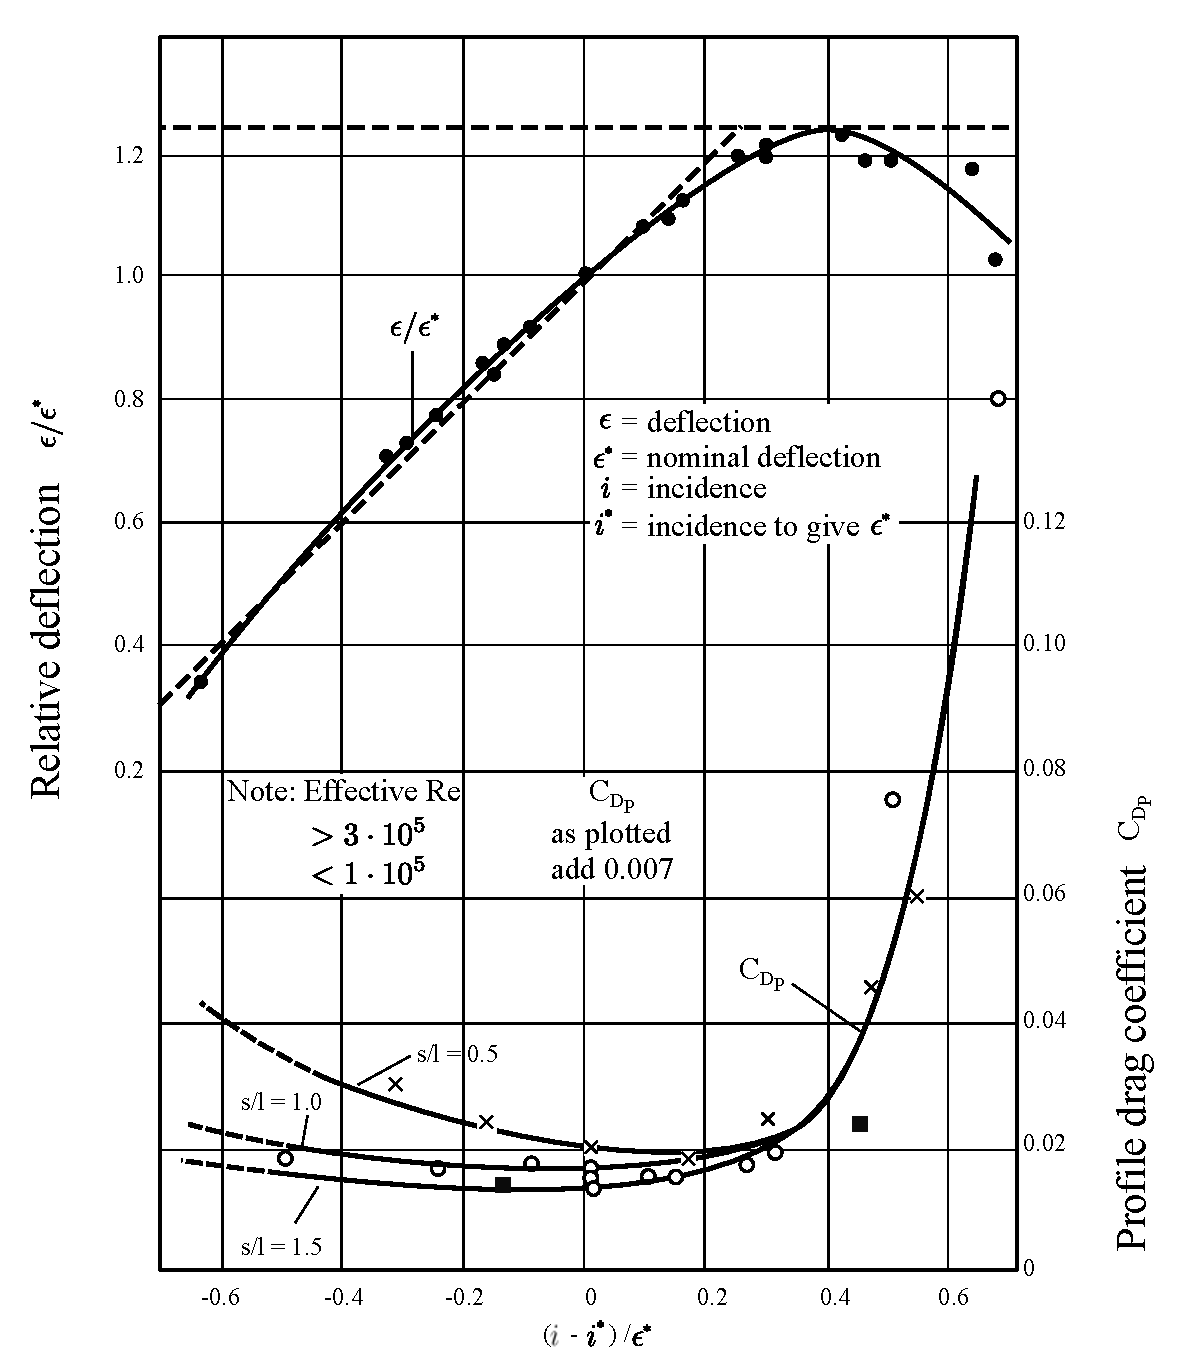
\includegraphics[width=0.8\textwidth]{fig/FuoriProg1.pdf}
\caption{}
\label{fig:FuoriProg1}
\end{figure}
Il diagramma in figura \ref{fig:FuoriProg1} permette di stimare il coefficiente di perdita $c_{Dp}$ e di considerare eventuali campi di variazione di Re differenti da quelli studiati nelle precedenti correlazioni; le curve vengono espresse a differenti valori di solidità.\\
In figura \ref{fig:FuoriProg2} si rapporta il coefficiente di incremento di pressione e il numero di Mach in entrata per una schiera con le caratteristiche riportate in figura; in questo modo è possibile avvicinarsi alle condizioni soniche e considerare anche i fenomeni di comprimibilità.
\begin{figure}[h!]
\centering
\begin{minipage}{.6\textwidth}
  \centering
  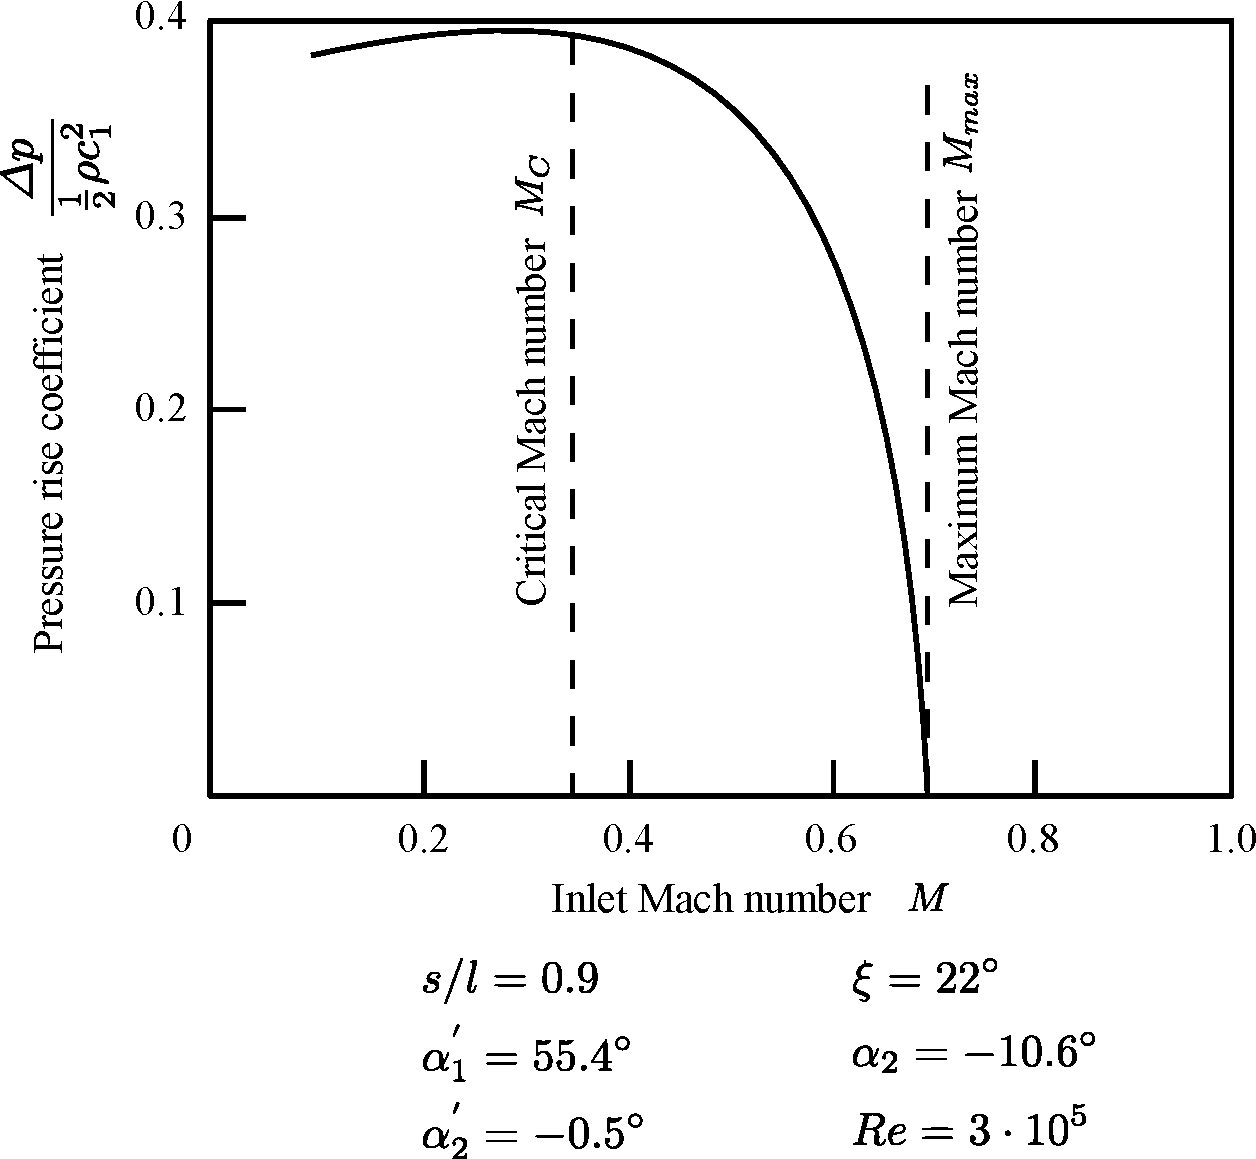
\includegraphics[width=.95\linewidth]{fig/FuoriProg2.pdf}
  \captionof{figure}{}
  \label{fig:FuoriProg2}
\end{minipage}%
\begin{minipage}{.4\textwidth}
  \centering
  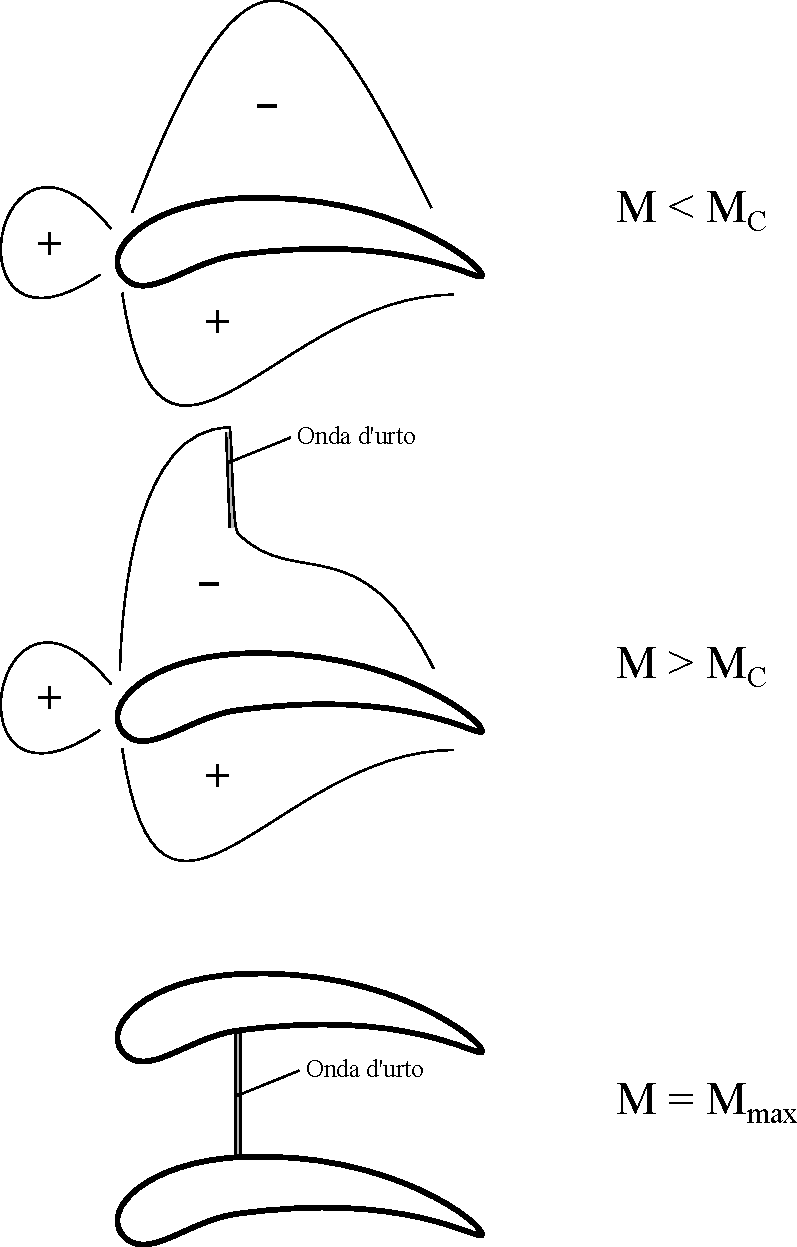
\includegraphics[width=.95\linewidth]{fig/FuoriProgMach.pdf}
  \captionof{figure}{ Campo di pressione attorno al profilo al variare del numero di Mach}
  \label{fig:FuoriProgMach}
\end{minipage}
\end{figure}
\\Finchè Ma resta basso il coefficiente di recupero di pressione non dipende da Ma. Raggiunto il valore di $M_{critico}$ il coefficiente di recupero di pressione diminuisce e c'è la possibilità che si formi un'onda d'urto con un decadimento delle prestazioni della schiera fino ad arrivare al loro annullamento in corrispondenza di $M_{max}$; in quest'ultima condizione in particolare, si ha un'onda d'urto che occupa l'intero condotto, quindi con condizioni di chocking, e di conseguenza la portata non può variare. La maggior parte dei test sperimentali che vengono svolti hanno lo scopo di trovare $M_c$.
\begin{figure}[h!]
	\centering
	\begin{minipage}{.6\textwidth}
		\centering
		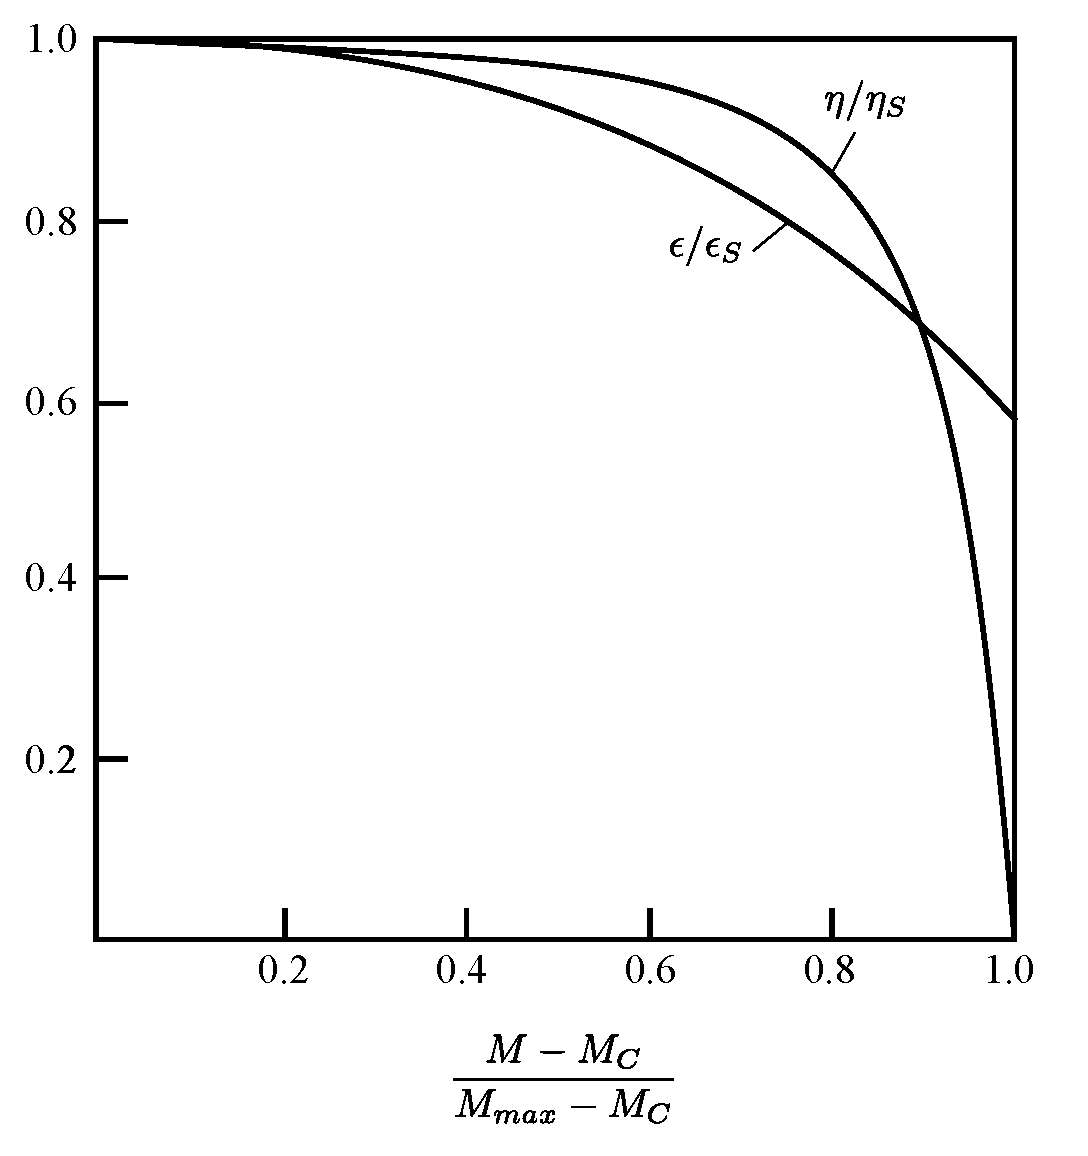
\includegraphics[width=\linewidth]{fig/FuoriProg3.pdf}
		\captionof{figure}{}
		\label{fig:FuoriProg3}
	\end{minipage}%
	\begin{minipage}{.4\textwidth}
		\centering
		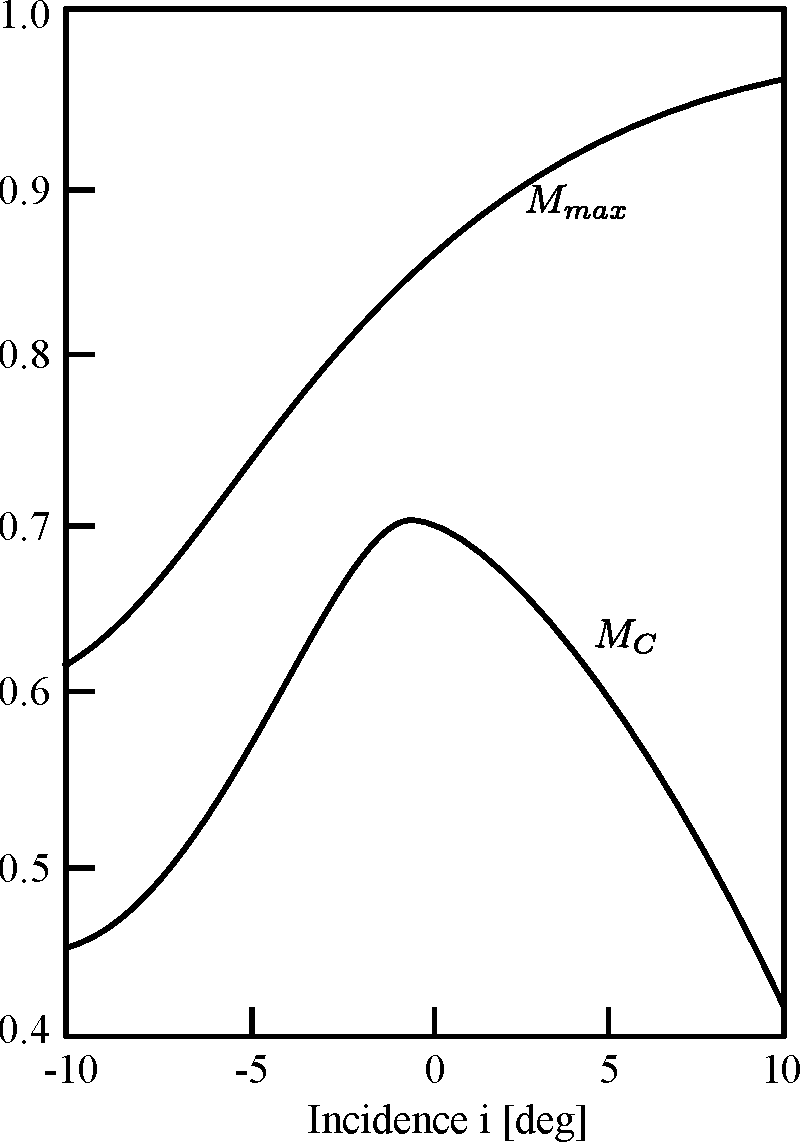
\includegraphics[width=\linewidth]{fig/FuoriProg4.pdf}
		\captionof{figure}{}
		\label{fig:FuoriProg4}
	\end{minipage}
\end{figure}
\\In figura \ref{fig:FuoriProg3} sono riportate le relazioni che correlano deflessione della schiera e il rendimento in funzione di una grandezza dipendente da $M$, $M_C$ e $M_{max}$ (sono valori specifici per condizioni fissate). \'E possibile notare dalla figura \ref{fig:FuoriProg4} come soprattutto $M_C$ sia pesantemente influenzato dall'angolo di incidenza.

\subsection{Criterio di carico}
Al variare del numero di pale ma a parità di lavoro svolto dalla macchina, si dovranno imporre diverse deflessioni con un conseguente carico diverso sulla singola pala: con poche pale si dovranno imporre deflessioni maggiori che portano ad un forte carico sul singolo profilo.\\
Si fa quindi una verifica: fissata la schiera e la solidità, si calcola il coefficiente di deflessione locale, $D_{loc}$, che indica quant'è la massima decelerazione a cui è soggetta la schiera:
\begin{equation}\label{eq:D_loc}
D_{loc} = \frac{V_{max} - V_2}{V_{max}}
\end{equation}
Si considera poi la riduzione di quantità di moto integrando sullo spessore occupato dalla scia:
\begin{equation}\label{eq:D_ridqmot}
\theta = \int_{\delta_P}^{\delta_S} \frac{\nu}{V} \bigg(1- \frac{\nu}{V} \bigg) dy
\end{equation} 
con $V$ è velocità di riferimento e $\nu$ velocità come funzione della posizione.
\begin{figure}
\centering
  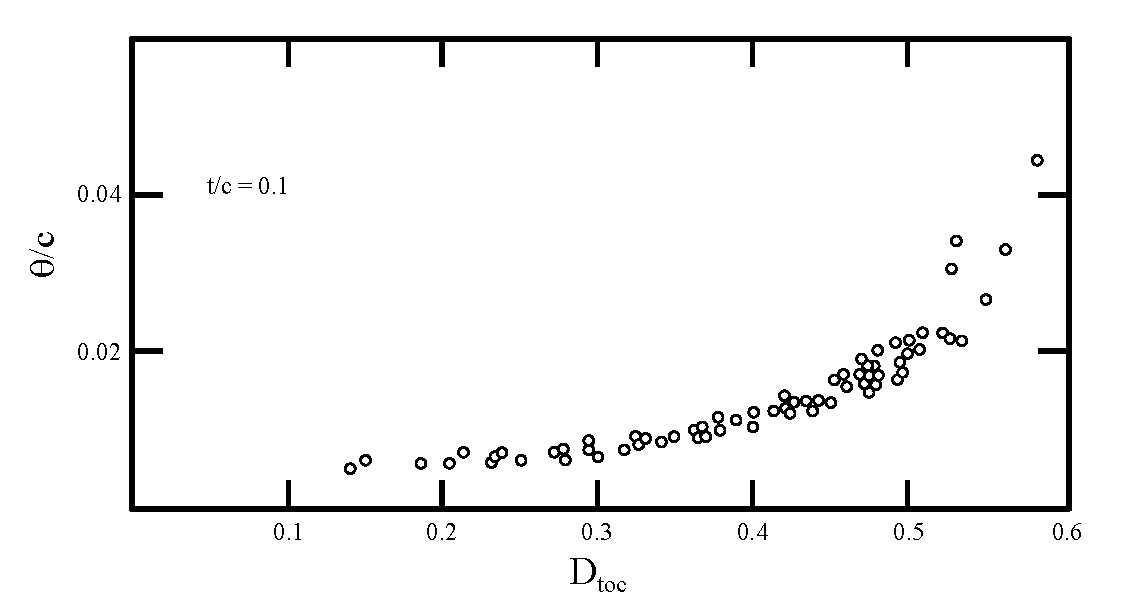
\includegraphics[width=\textwidth]{fig/CritCarico1.pdf}
\caption{}
\label{fig:CritCarico1}
\end{figure}
\begin{figure}
\centering
  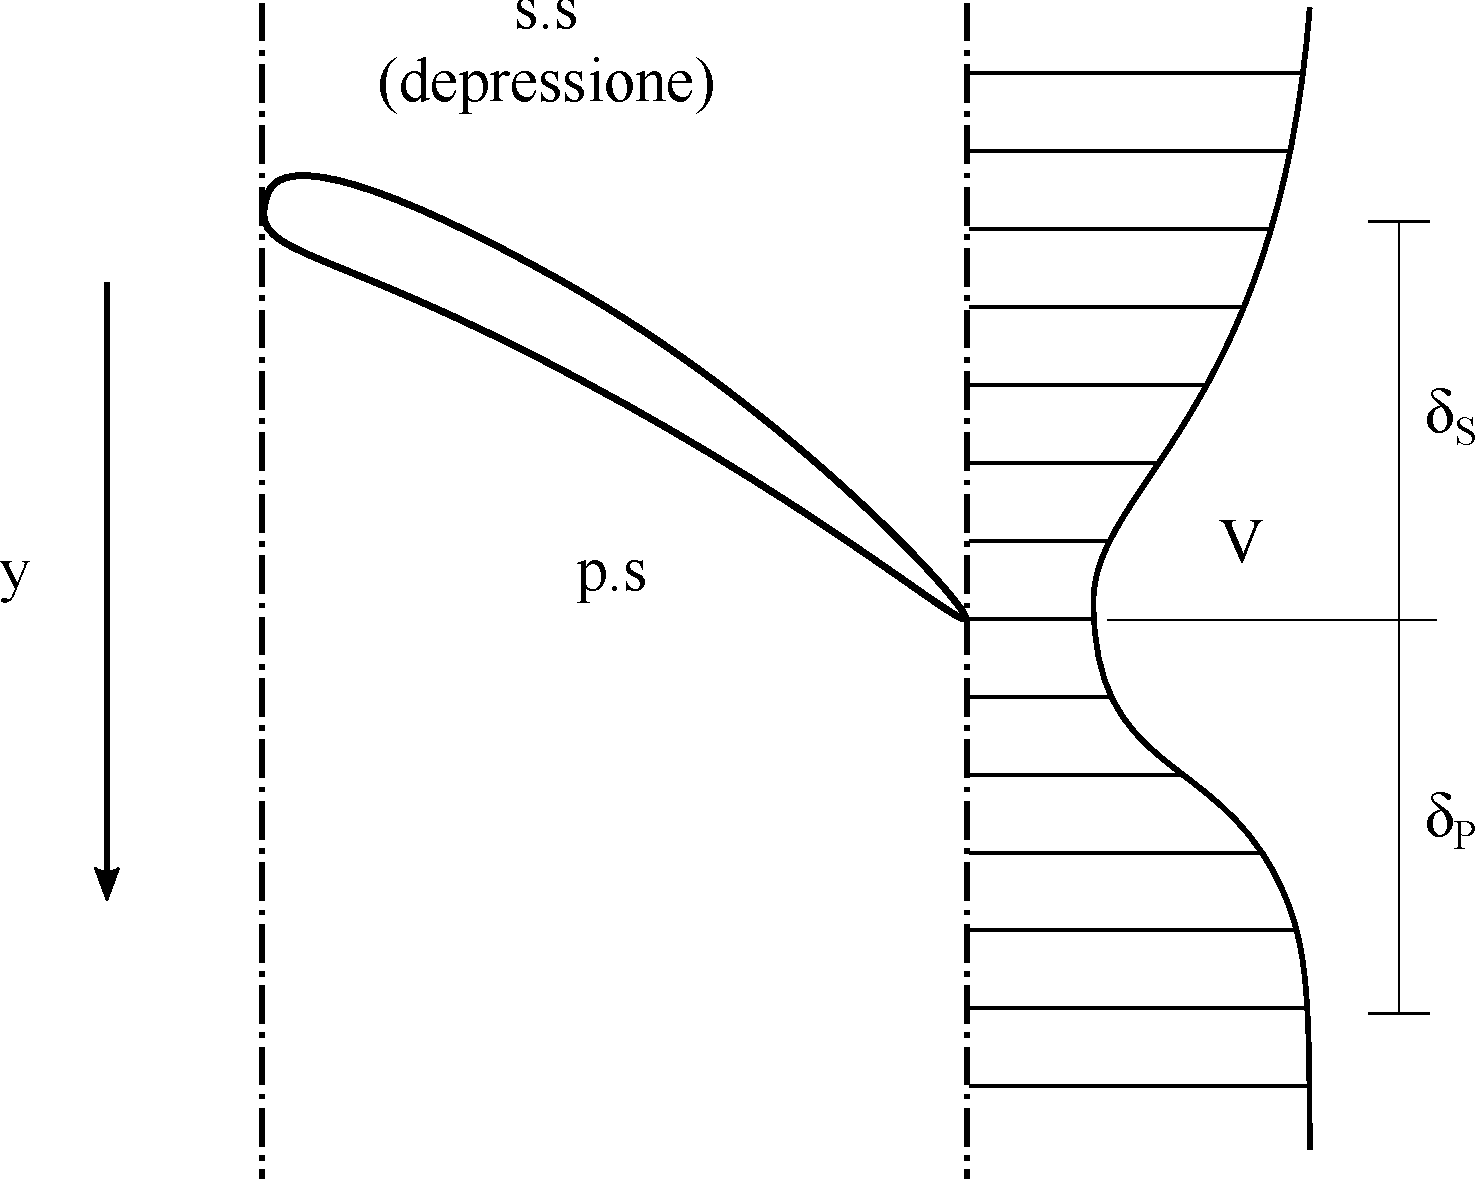
\includegraphics[width=.4\textwidth]{fig/CritCarico2.pdf}
\caption{}
\label{fig:CritCarico2}
\end{figure}
Se sono presenti molte pale, l'integrale diventa molto grande perché l'intero canale palare potrebbe essere occupato dalla scia, quindi come criterio empirico si utilizza:
\begin{align*}
\frac{\theta}{c} < 0.2
\end{align*}
In questo modo l'inspessimento di strato limite è considerato trascurabile rispetto alla corrente principale. 
\begin{figure}
\centering
  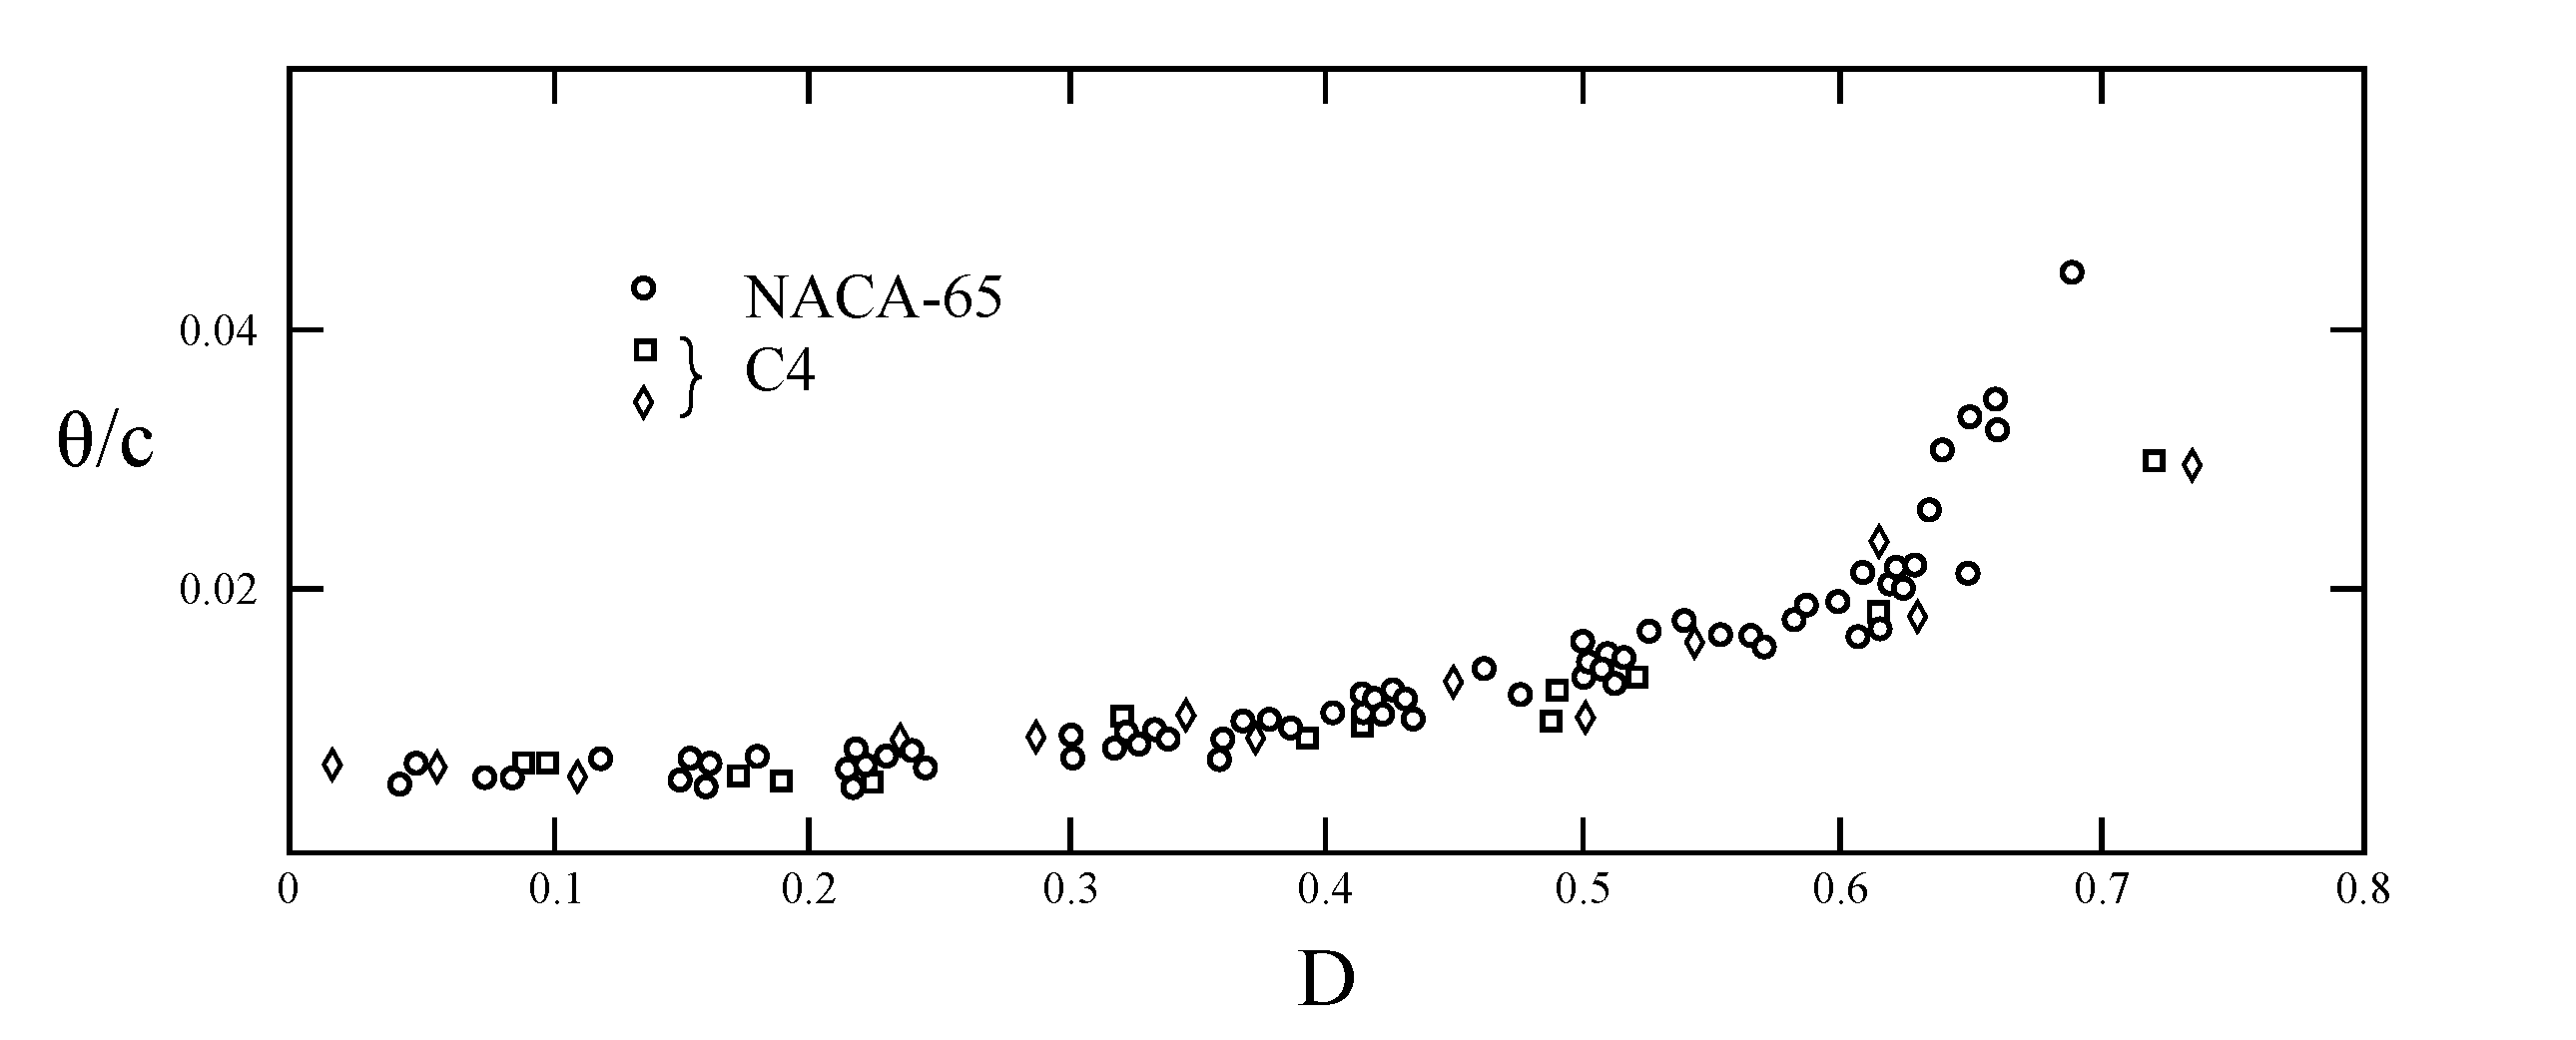
\includegraphics[width=\textwidth]{fig/CritCarico3.pdf}
\caption{}
\label{fig:CritCarico3}
\end{figure}
\\\'E possibile calcolare un fattore di diffusione globale, $D$, attraverso differenti correlazioni ottenute a partire da dati sperimentali (figura \ref{fig:CritCarico3}):
\begin{align*}
D = \bigg( \frac{V_1 - V_2}{V_1} \bigg) + \bigg( \frac{V_{t1} - V_{t2}}{2 \sigma V_1} \bigg) = \bigg( 1 - \frac{\cos \alpha_1}{cos \alpha_2} \bigg) + \frac{\cos \alpha_1}{2 \sigma} (\tan \alpha_1 - \tan \alpha_2)
\end{align*}
e come criterio empirico si usa $ D \leqslant 0.4 \div 0.5  $.
\begin{figure}
\centering
  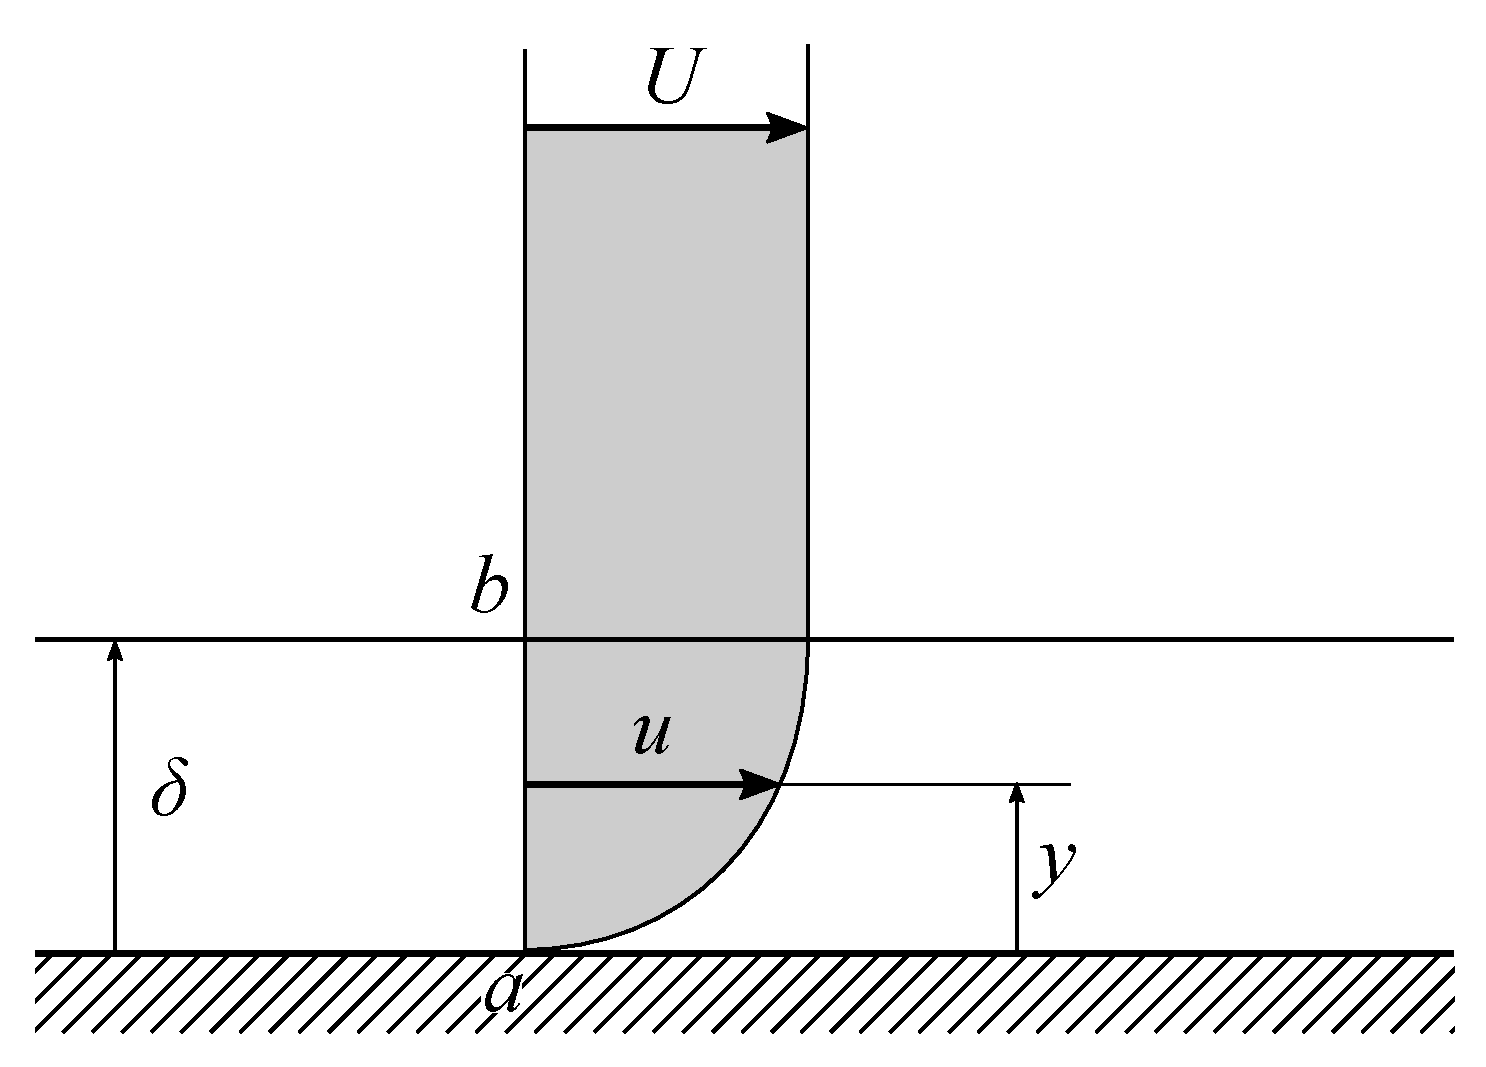
\includegraphics[width=.4\textwidth]{fig/CritCarico4.pdf}
\caption{}
\label{fig:CritCarico4}
\end{figure}
\\Infine si possono andare a cercare correlazioni rispetto allo strato limite come mostrato in figura \ref{fig:CritCarico4} e calcolare il decremento della quantità di moto come 
\begin{align*}
\Delta M = \int_0^{\delta} \rho u dy (U-u) = \rho \int_0^{\delta} u (U-u) dy
\end{align*} 
Quest'ultima fase però attualmente non ha molto senso in quanto questa è la parte di progettazione che si effettua per via numerica. A partire da questo decremento, è possibile calcolare lo spessore della quantità di moto dello strato limite al fine di valutare l'intensità energetica della scia in termini di perturbazione:
\begin{equation}
\theta = \frac{\Delta M}{\rho U^2} = \int_0^{\delta} \frac{u}{U} \bigg( 1 -\frac{u}{U} \bigg) dy
\end{equation}

\section{Schiere supersoniche}
Fin'ora si sono analizzate schiere di compressori con deflusso subsonico debolmente comprimibile con rapporti di compressione modesti ($10 \div 20 \%$) e con le seguenti condizioni sulla velocità in ingresso e in uscita:
\begin{align*}
\begin{cases}
M_1 <1\\
M_2 <1
\end{cases}
\end{align*} 

Si analizzano ora delle condizioni diverse in cui si presenteranno condizioni supersoniche. Questo tipo di deflusso consente un salto di pressione più elevato a scapito però di una pesante perdita in termini di rendimento. Queste trovano applicazioni particolari in campo aeronautico. 
\begin{itemize}
	\item Si parlerà di compressore transonico se:
	\begin{align*}
	\begin{cases}
	M_1 >1\\
	M_2 <1
	\end{cases}
	\end{align*} 
	Nel caso in cui si arrivi in condizione soniche all'interno della macchina si faranno ulteriori distinzioni rispetto alla componente assiale: 
	\begin{itemize}
		\item per $M_{1a} < 1 $ si parlerà di:
		\begin{itemize}
			\item \textit{regime non innescato} (figura \ref{fig:Schlieren1}a): è presente un'onda d'urto normale al flusso. Si avrà quindi una zona supersonica a monte e una subsonica a valle della schiera con un passaggio tra le due discontinuo; l'aumento di velocità è dovuto all'aumento di spessore della schiera;
			\item \textit{regime innescato} (figura \ref{fig:Schlieren1}b): la perturbazione di pressione occupa integralmente il condotto palare ed è distinguibile in maniera chiara (è comunque presente una zona subsonica in ingresso); la portata è bloccata; 
		\end{itemize}
		\item per $ M_{1a} > 1 $ si parlerà di \textit{regime saturo} (figura \ref{fig:Schlieren1}c): il blocco sonico è a monte della schiera dove si creano delle onde oblique che dissipano energia. Il deflusso in questo caso è complesso;
	\end{itemize}
	\item un'ulteriore possibilità, che però non ha rilevanza nei compressori, è:
	\begin{align*}
	\begin{cases}
	M_1 <1\\
	M_2 >1
	\end{cases}
	\end{align*} 
	In questo caso il flusso viene accelerato ma per definizione in un compressore si cerca esattamente l'effetto opposto;
	\item un ultimo caso è:
	\begin{align*}
	\begin{cases}
	M_1 >1\\
	M_2 >1
	\end{cases}
	\end{align*} 
	in cui il flusso è interamente supersonico ma non ha particolari interessi applicativi.
\end{itemize}
\begin{figure}[h!]
\centering
  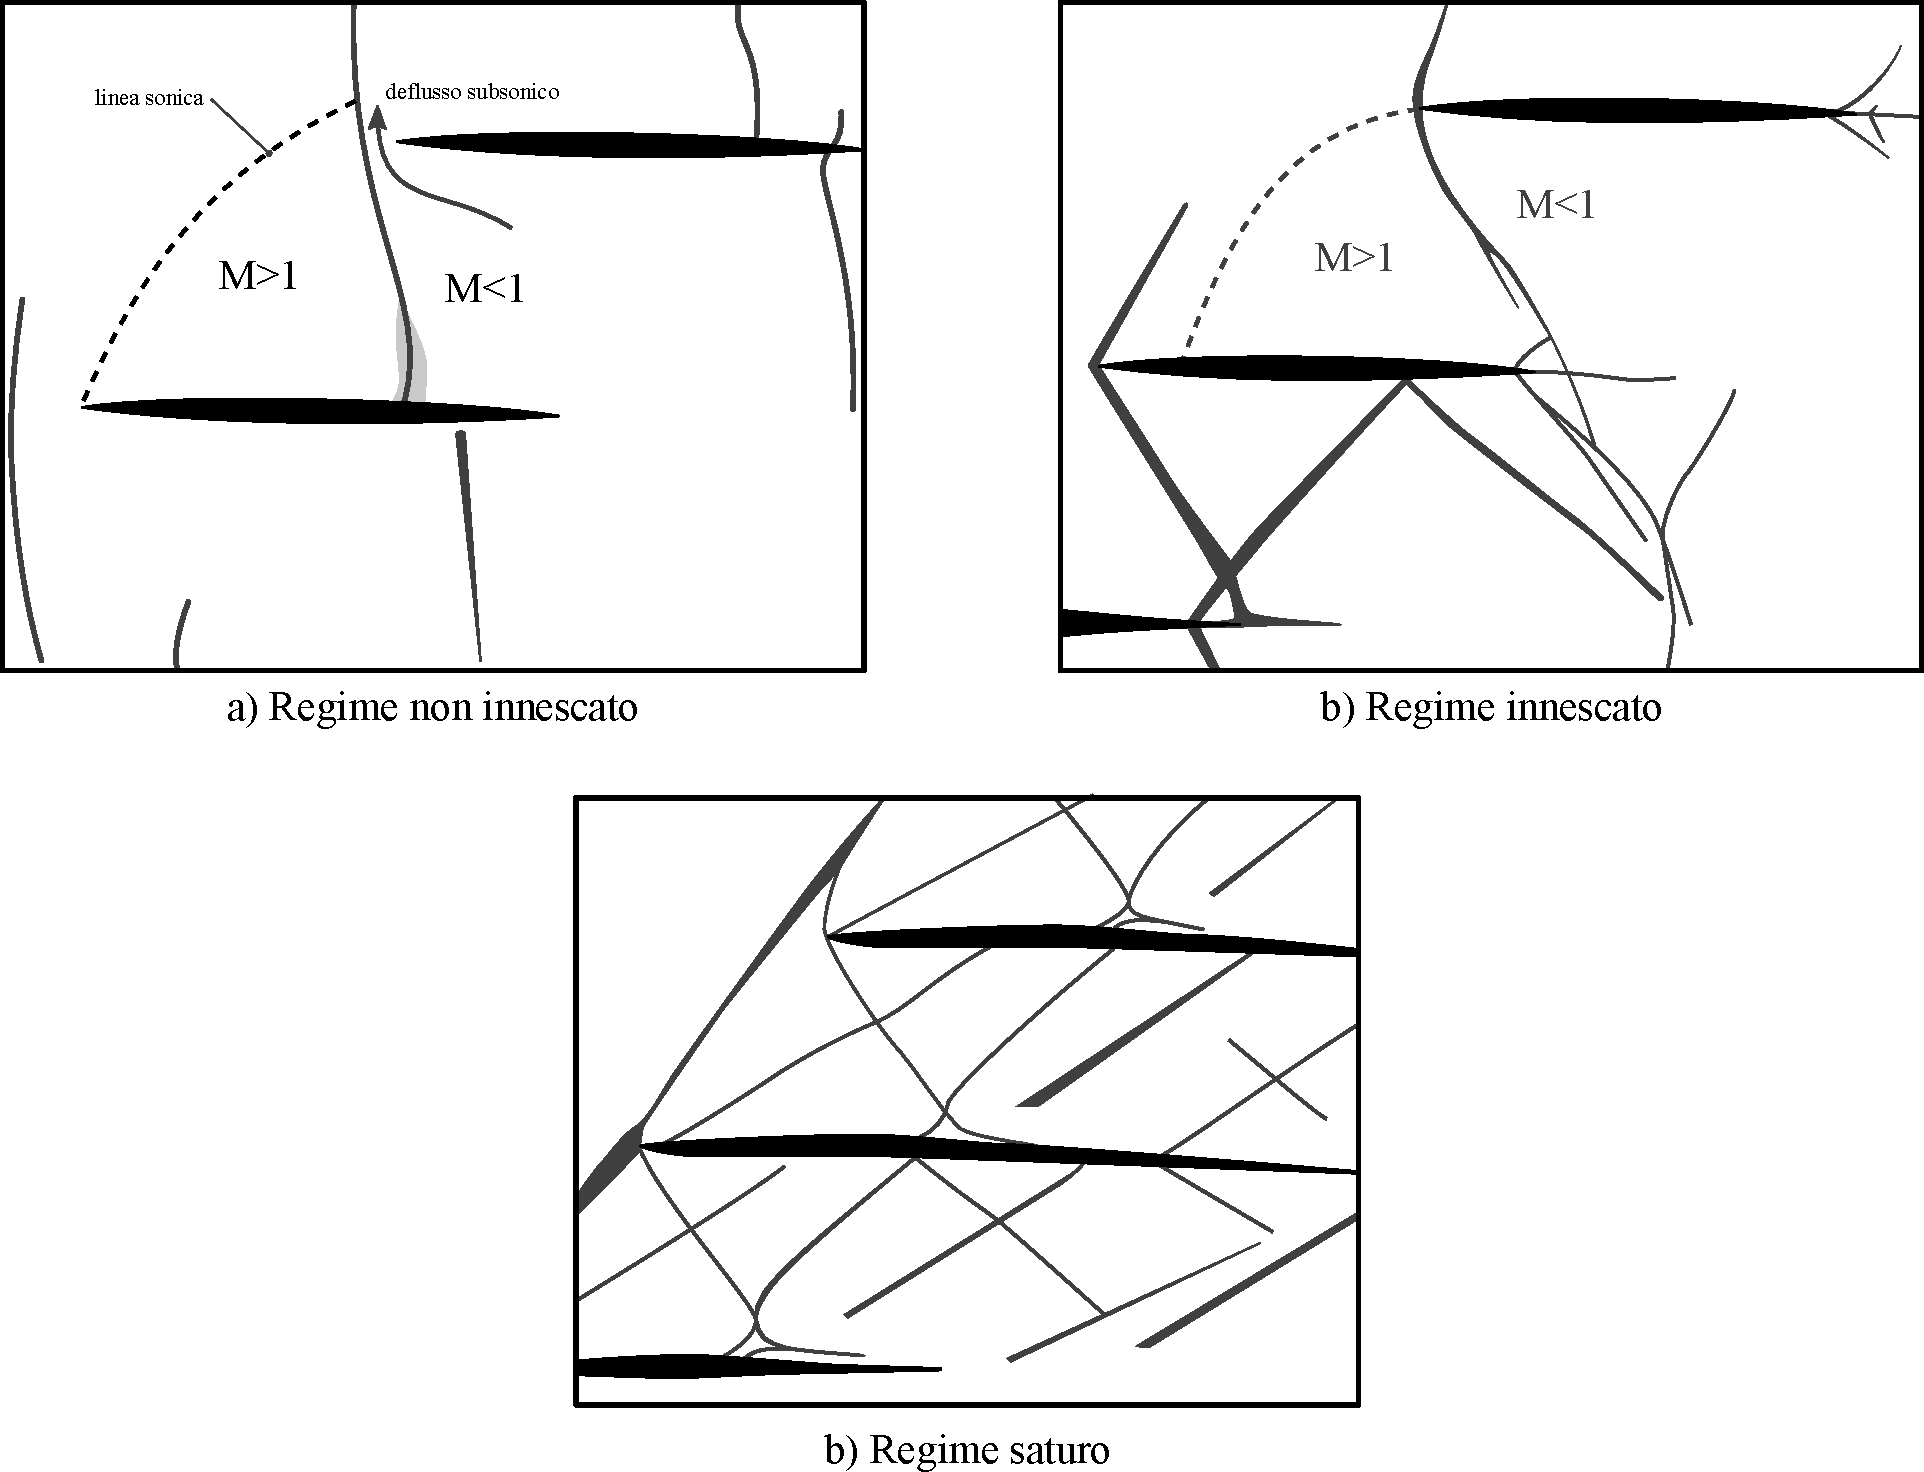
\includegraphics[width=.8\textwidth]{fig/Schlieren1.pdf}
\caption{}
\label{fig:Schlieren1}
\end{figure}
\begin{figure}[h!]
\centering
  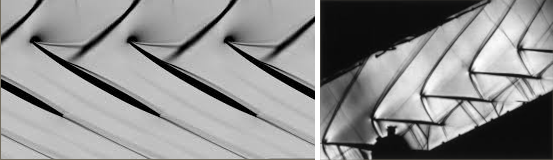
\includegraphics[width=.8\textwidth]{fig/Schlieren2.png}
\caption{}
\label{fig:Schlieren2}
\end{figure}
